\documentclass{article}
\usepackage[a4paper, top=1in, bottom=1in, left=1in, right=1in]{geometry}
\usepackage[utf8]{inputenc}

\usepackage[english]{babel}
\usepackage{tikz-cd, extarrows, esvect, esint, pgfplots, lipsum, bm, dcolumn}
\usetikzlibrary{arrows}
\usepackage{amsmath, amssymb, amsthm, mathrsfs, mathtools, centernot, hyperref, fancyhdr, lastpage}


\renewcommand{\thispagestyle}[1]{}

\DeclareMathOperator{\Tr}{Tr}
\DeclareMathOperator{\Sym}{Sym}
\DeclareMathOperator{\Span}{span}
\DeclareMathOperator{\im}{Im}
\DeclareMathOperator{\Div}{div}
\DeclareMathOperator{\curl}{curl}
\DeclareMathOperator{\GL}{GL}
\DeclareMathOperator{\SL}{SL}
\DeclareMathOperator{\GA}{GA}
\DeclareMathOperator{\std}{std}
\DeclareMathOperator{\Cov}{Cov}
\DeclareMathOperator{\Var}{Var}
\DeclareMathOperator{\Corr}{Corr}
\DeclareMathOperator{\Int}{Int}
\DeclareMathOperator{\Id}{Id}
\DeclareMathOperator{\Lie}{Lie}
\DeclareMathOperator{\Hom}{Hom}
\DeclareMathOperator{\Alt}{Alt}
\DeclareMathOperator{\rank}{rank}
\DeclareMathOperator{\conv}{conv}
\DeclareMathOperator{\aff}{aff}
\DeclareMathOperator{\arccot}{arccot}


\newtheorem{theorem}{Theorem}[section]
\newtheorem{proposition}[theorem]{Proposition}
\newtheorem{lemma}[theorem]{Lemma}
\newtheorem{example}{Example}[section]
\newtheorem{corollary}{Corollary}[theorem]
\theoremstyle{remark}
\newtheorem*{remark}{Remark}
\theoremstyle{definition}
\newtheorem{definition}{Definition}[section]
\renewcommand{\qed}{\hfill$\blacksquare$}
\renewcommand{\footrulewidth}{0.4pt}% default is 0pt


\begin{document}
\pagestyle{fancy}

\lhead{Probability}
\chead{Muchang Bahng}
\rhead{\date{August 2021}}
\cfoot{\thepage / \pageref{LastPage}}

\title{Probability}
\author{Muchang Bahng}
\date{November 2022}

\maketitle

An abstract introduction to probability and its applications. 

\section{Probability Spaces}
In order to define a probability space, we must revisit a concept in algebra. 

\begin{definition}
A \textbf{$\sigma$-algebra} (or a \textbf{$\sigma$-field}) on a set $X$ is a collection $\Sigma$ of subsets fo $X$ that includes $X$ itself, is closed under complement, and is closed under countable unions. 

This definition implies that $\emptyset \in X$, and $\Sigma$ is closed under countable intersections. Furthermore, a $\sigma$-algebra is a type of algebra of sets. 
\end{definition}

\begin{example}
Given any set $X$, $2^X$ is a $\sigma$-algebra. 
\end{example}

\begin{example}
A $\sigma$-algebra $\mathcal{F} \subseteq 2^{\Omega}$ corresponds to a finite or countable partition $\Omega = B_1 \cup B_2 \cup \ldots$, with the general form of an event $A \in \mathcal{F}$ being 
\[A = B_{k_1} \cup B_{k_2} \cup \ldots \]
\end{example}

\begin{definition}
A \textbf{measure} on a set is a systematic way to assign a number, intuitively interpreted as its "size," to some subsets of that set, called \textbf{measurable sets}. That is, let $X$ be a set and $\Sigma$ be a $\sigma$-algebra over $X$. A function $\mu: \Sigma \longrightarrow \mathbb{R} \cup \{\infty, -\infty\}$ is called a measure if it satisfies the following properties: 
\begin{enumerate}
    \item Non-negativity: For all $E \in \Sigma$, we have $\mu (E) \geq 0$. 
    \item Null empty set: $\mu (\emptyset) = 0$
    \item Countable additivity: For all countable collections $\{E_k\}_{k=1}^\infty$ of pairwise disjoint sets in $\Sigma$, 
    \[\mu \bigg( \bigsqcup_{k=1}^\infty E_k \bigg) = \sum_{k=1}^\infty \mu (E_k)\]
\end{enumerate}
If at least one set $E$ has finite measure, then the requirement that $\mu (\empty) = 0$ is met automatically. Indeed, by countable additivity, 
\[\mu(E) = \mu(E \cup \emptyset) = \mu(E) + \mu(\emptyset) \implies \mu(\emptyset) = 0\]
\end{definition}

\subsubsection{Lebesgue Measure}
A popular measure and one that is a generalization of our natural notions of length, area, and volume is the \textit{Lebesgue measure}. To properly introduce the motivation for this measure, we recognize the need to measure the "size" of a set in $\mathbb{R}$. For intervals $I = (a, b)$, we can simply use the length $l$ defined as 
\[l(I) \equiv b - a, \;\;\; \text{ where } a \leq b\]
However, if we are measuring the set of, say, all irrational numbers in $\mathbb{R}$, this notion of length fails us. Therefore, we must extend this concept of length/size of an interval to arbitrary sets. Given a set $E$ of real numbers, let $\lambda(E)$ represent its Lebesgue measure, which should have properties: 
\begin{enumerate}
    \item If $I$ is an interval, then $\lambda(I)$ should naturally be $l(I)$. 
    \item If $A \subset B$, then $\lambda (A) \leq \lambda(B)$. 
    \item Given $A \subset \mathbb{R}$ and $x_0 \in \mathbb{R}$, define $A + x_0 \equiv \{x + x_0\,|\, x \in A\}$, the translation of $A$. Then $\lambda (A + x_0) = \lambda (A)$, since translation should not change the measure. 
    \item If $A, B$ are disjoint sets, then $\lambda(A \cup B) = \lambda(A) + \lambda(B)$. That is, if $\{A_i\}_{i \in \mathbb{N}}$ is a sequence of disjoint sets, then 
    \[\lambda \bigg( \bigcup_{i=1}^\infty A_i\bigg) = \sum_{i=1}^\infty \lambda(A_i)\]
\end{enumerate}
However, it is a fact that it is \textit{not} possible to define a measure that satisfies all of these properties for all subsets of real numbers. The difficulty lies in property $4$, which is essential to guarantee the linearity of the Lebesgue integral. In other words, some sets will not have a Lebesgue measure, that is, are not Lebesgue measurable. 

\begin{definition}
Let $E \subseteq \mathbb{R}$. The \textbf{Lebesgue outer measure} of $E$, denoted by $\lambda^* (E)$, is defined
\[\lambda^*(E) \equiv \inf \bigg\{ \sum_k l(I_k)\,|\,\{I_k\} \text{ is a sequence of open intervals with } E \subseteq \bigcup_k I_k \bigg\}\]
In other words, $\cup_{k} I_k$ is a cover of $E$. Clearly, $0 \leq \lambda^* (E) \leq \infty$.
\end{definition}

\begin{lemma}[Properties of the Lebesgue Outer Measure]
$\lambda^*$ has the following properties: 
\begin{enumerate}
    \item If $A \subseteq B$, then $\lambda^* (A) \leq \lambda^*(B)$. 
    \item $\lambda^* (\emptyset) = 0$. 
    \item If $A$ is a countable set, then $\lambda^* (A) = 0$. 
    \item Lebesgue outer measure is invariant under translation. That is, for each $x_0 \in \mathbb{R}$, $\lambda^* (E + x_0) = \lambda^* (E)$. 
    \item Lebesgue outer measure is countably subadditive. That is, given a sequence of sets $\{E_i\}$, 
    \[\lambda^* \bigg( \bigcup_i E_i \bigg) \leq \sum_i \lambda^* (E)\]
    \item For any interval $I$, $\lambda^* (I) = l(I)$.
\end{enumerate}
\end{lemma}

With this definition, every set has a Lebesgue outer measure and satisfies the properties 1-3 mentioned before. However, it is not guaranteed to satisfy property 4, as there exists two disjoint sets $A, B$ for which $\lambda^* (A \cup B) \neq \lambda^* (A) + \lambda^* (B)$. However, we will focus our attention on a collection of sets, known as measurable sets, for which property 4 holds. 

\begin{definition}
Let set $E \subseteq \mathbb{R}$ be \textbf{Lebesgue measurable} if for each set $A \subseteq \mathbb{R}$, it satisfies the \textit{Caratheodory criterion}, which requires that
\[\lambda^* (A) = \lambda^* (A \cap E) + \lambda^* (A \cap E^C)\]
where $E^C = \mathbb{R} \setminus E$. If $E$ is a Lebesgue measurable set, then the Lebesgue measure of $E$, denoted $\lambda(E)$ is defined to be its outer Lebesgue measure $\lambda^* (E)$. 

The \textbf{Lebesgue $\sigma$-algebra} is the collection of all sets $E$ which satisfy the Caratheodory criterion. As stated before, for any set in the Lebesgue $\sigma$-algebra, its Lebesgue measure is given by 
\[\lambda (E) \equiv \lambda^* (E)\]
\end{definition}

The intuition that characterises the Lebesgue outer measure can be seen as the \textit{total length of interval sets which fit $E$ most tightly and do not overlap}. Whether this outer measure translates to the Lebesgue measure proper depends on an additional condition. 

This condition is tested by taking subsets $A$ of the real numbers using $E$ as an instrument to split $A$ into two partitions: the part of $A$ which intersects with $E$ and the remaining part of $A$ which is not in $E$. These partitions of $A$ are subject to the outer measure. If for all possible such subsets $A$ of the real numbers, the partition of $A$ cut part by $E$ have outer measures whose sum is the outer measure of $A$, then the outer Lebesgue measure of $E$ gives its Lebesgue measure.

This condition means that the set $E$ must not have some curious properties which causes a discrepancy in the measure of another set when $E$ is used as a "mask" to "clip" that set. 

\begin{theorem}
There exists sets that are not Lebesgue measurable. 
\end{theorem}

\begin{example}
A \textbf{Vitali set} is a subset $V$ of the interval $[0,1]$ of $\mathbb{R}$ such that, for each real number $r$, there is exactly one number $v \in V$ such that $v=r$ is a rational number. It is known that a Vitali set is non-measurable. 
\end{example}

\begin{lemma}[Measurable sets]
The collection of measurable sets has the following properties: 
\begin{enumerate}
    \item $\emptyset$ and $\mathbb{R}$ are measurable. 
    \item If $E$ is measurable, then so is $E^C$. 
    \item If $\lambda^* (E) = 0$, then $E$ is measurable. 
\end{enumerate}
\end{lemma}

\begin{lemma}
Every open set and every closed set are measurable. 
\end{lemma}

\begin{definition}[Measurable vs Measure Spaces]
The pair $(X, \Sigma)$ ($X$ a set with $\Sigma$ its $\sigma$-algebra) is called a \textit{measurable space}, the members of $\Sigma$ are called measurable sets. Note that no measure is needed for measurable spaces. 

The triple $(X, \Sigma, \mu)$ is called a \textbf{measure space}. Unlike a measurable space, a measure space requires a measure function $\mu$. 
\end{definition}

\begin{definition}[Probability Space]
A \textbf{probability space} is a measure space such that the measure of the space is equal to $1$. More specifically, it is a triple $(\Omega, \mathcal{F}, P)$ consisting of: 
\begin{enumerate}
    \item The \textbf{sample space} $\Omega$ is the set of all possible outcomes, where an \textbf{outxome} is the result of a single execution of the model. 
    \item The \textbf{event space} $F \subseteq 2^{\Omega}$, which is a $\sigma$-algebra and the set of subsets of $\Omega$. Each element of $\mathcal{F}$ is called an \textbf{event}, with each event being a set of outcomes in the sample space. Note that since $\mathcal{F}$ is a $\sigma$-algebra, 
    \begin{enumerate}
        \item $\mathcal{F}$ contains the sample space: $\Omega \in \mathcal{F}$
        \item $\mathcal{F}$ is closed under complements: $A \in \mathcal{F} \implies (\Omega \setminus A) \in \mathcal{F}$
        \item $\mathcal{F}$ is closed under countable unions and countable intersections
        \[A_1, \ldots \in \mathcal{F} \implies \bigcup_{i=1}^\infty A_i \in \mathcal{F}, \bigcap_{i=1}^\infty A_i \in \mathcal{F}\]
    \end{enumerate}
    An event is considered to have \textit{happened} during an experiment when the outcome of the model is an element of the event. Since the same outcome may be a member of many events, it is possible for many events to have happened given a single outcome. 
    \item The probability measure $P: \mathcal{F} \longrightarrow [0,1]$ is a function returning an event's probability, such that
    \begin{enumerate}
        \item $P$ is countably additive. That is, if $\{A_i\}_{i=1}^\infty$ is a countable collection of pairwise disjoint sets, then 
        \[P \bigg( \bigcup_{i=1}^\infty A_i \bigg) = \sum_{i=1}^\infty P(A_i)\]
        \item The measure of the entire sample space equals $1$
        \[P(\Omega) = 1\]
    \end{enumerate}
\end{enumerate}
Note that not every subset of the sample space $\Omega$ must necessarily be considered an event: some of the subsets are simply not of interest, and others cannot be measured. This is not so obvious in a case like a coin toss. In a different example, one could consider javelin throw lengths, where the events typically are intervals like "between $60$ and $65$ meters" and unions of such intervals, but not sets like the "irrational numbers between $60$ and $65$ meters".
\end{definition}

Using countable additivity, we can see that given two events $A, B \in \mathcal{F}$, 
\[A \subset B \implies \mathbb{P}(A) \leq \mathbb{P}(B)\]
Intuitively, this means that if the cases in $B$ contains all the cases in $A$, the probability of a case being in $B$ is at least that of a case being in $A$. 

\subsection{Discrete Case}
Discrete probability theory needs only at most countable sample spaces $\Omega$. Probabilities can be ascribed to points of $\Omega$ by the probability mass function $p: \Omega \longrightarrow [0,1]$ such that
\[\sum_{\omega \in \Omega} p(\omega) = 1\]
All subsets of $\Omega$ can be treated as events, making $\mathcal{F} = 2^{\Omega}$. The probability measure takes the simple form 
\[P(A) = \sum_{\omega \in A} p(\omega) \text{ for all } A \subseteq \Omega\]
The greatest $\sigma$-algebra $F = 2^{\Omega}$ describes the complete information. The cases $p(\omega) = 0$ is permitted by the definition, but rarely used since such $\omega$ can safely be excluded from the sample space. 

\begin{example}
Consider the flip of a fair coin with outcomes either hands or tails. Then, $\Omega = \{H, T\}$. The $\sigma$-algebra $F = 2^{\Omega}$ contains $2^2 = 4$ events: 
\begin{align*}
    \{\} &= \text{Neither heads nor tails} \\
    \{H\} &= \text{Heads} \\
    \{T\} &= \text{Tails} \\
    \{H, T\} &= \text{Either heads or tails}
\end{align*}
That is, $\mathcal{F} = \{\{\}, \{H\}, \{T\}, \{H, T\}\}$. Our probability measure $P$ is defined
\[P(f) = \begin{cases}
0 & f = \{\} \\
0.5 & f = \{H\} \\
0.5 & f = \{T\} \\
1 & f = \{H, T\}
\end{cases}\]
\end{example}

\begin{example}
A fair coin is tossed 3 times, creating 8 possible outcomes. 
\[\Omega = \{HHH, HHT, HTH, HTT, THH, THT, TTH, TTT\}\]
The complete information is described by the $\sigma$-algebra $\mathcal{F} = 2^{\Omega} = 2^8 = 256$ events, where each of the events is a subset of $\Omega$. 

Alice knows the outcome of the second toss only. Thus, her incomplete information is described by the partition 
\[\Omega = A_1 \sqcup A_2 = \{HHH, HHT, THH, THT\} \sqcup \{HTH, HTT, TTH, TTT\}\]
and the corresponding $\sigma$-algebra is 
\[\mathcal{F}_{Alice} = \{\emptyset, A_1, A_2, \Sigma\}\]
Bryan knows only the total number of tails, so his partition contains 4 parts: 
\begin{align*}
    \Omega & = B_0 \sqcup B_1 \sqcup B_2 \sqcup B_3 \\
    & = \{HHH\} \sqcup \{HHT, HTH, TTH\} \sqcup \{TTH, THT, HTT\} \sqcup \{TTT\}
\end{align*}
When we calculate Bryan's event space, we have
\begin{align*}
    \mathcal{F}_{Bryan} & = \big\{\emptyset, \{HHH\}, \{HHT\}, \{HTH\}, \{THH\}, \{HHT, HTH\}, \{HHT, THH\}, \\
    & \;\;\;\;\{TTH, THT\}, \{TTH\}, \{THT\}, \{HTT\}, \{TTH, THT\},\{TTH, HTT\}, \\
    & \;\;\;\;\{THT, HTT\}, \{TTT\}, \Omega \big\} 
\end{align*}
Note that the event space of Bryan (and Alice) is not merely just $2^{\Omega}$ since we have some predetermined knowledge of the outcome space $\Omega$. Therefore, we can partition it into 4 cases and construct the event space by putting only the events that are subsets of each partition. For example, it wouldn't make sense to have an event 
\[\{HHH, TTT\}\]
since the events $\{HHH\}$ and $\{TTT\}$ are in completely different outcome spaces (given the number of tails). That is, if we knew that 3 tails were thrown, the event $\{HHH, TTT\}$ wouldn't make any sense. However, the event $\Omega$ or $\emptyset$ is viable since they describe the case of whether the coin was tossed at all or not. 
Furthermore, $\mathcal{F}_{Alice}$ and $\mathcal{F}_{Bryan}$ are incomparable. That is, $\mathcal{F}_{Alice} \not\subseteq \mathcal{F}_{Bryan}$ and $\mathcal{F}_{Bryan} \not\subseteq \mathcal{F}_{Alice}$, even though both are subalgebras of $2^{\Omega}$. 
\end{example}

\begin{example}
If $100$ voters are to be drawn randomly from among all voters in California and asked whom they will vote for governor, then the set of all sequences of $100$ Californian voters would be the sample space $\Omega$. We assume that sampling without replacement is used: only sequences of $100$ different voters are allowed. For simplicity an ordered sample is considered, that is a sequence $\{Alice, Bryan\}$ is different from $\{Bryan, Alice\}$. We also take for granted that each potential voter knows exactly his/her future choice, that is he/she doesn’t choose randomly.

Alice knows only whether or not Arnold Schwarzenegger has received at least $60$ votes. Her incomplete information is described by the $\sigma$-algebra $\mathcal{F}_{Alice}$ that contains:
\begin{enumerate}
    \item the set of all sequences in $\Omega$ where at least $60$ people vote for Schwarzenegger
    \item the set of all sequences where fewer than $60$ vote for Schwarzenegger
    \item the whole sample space $\Omega$
    \item the empty set $\emptyset$
\end{enumerate}
Bryan knows the exact number of voters who are going to vote for Schwarzenegger. His incomplete information is described by the corresponding partition $\Omega = B_0 \sqcup B_1 \ldots B_{100}$ and the $\sigma$-algebra $\mathcal{F}_{Bryan}$ consists of $2^{101}$ events. 

In this case Alice’s $\sigma$-algebra is a subset of Bryan’s: $\mathcal{F}_{Alice} \subset \mathcal{F}_{Bryan}$. Bryan’s $\sigma$-algebra is in turn a subset of the much larger "complete information" $\sigma$-algebra $2^{\Omega}$ consisting of $2^{n(n-1)\ldots (n-99)}$ events, where $n$ is the number of all potential voters in California. 
\end{example}

\subsection{General and Non-Atomic Cases}

\begin{definition}
Let $\Omega$ be uncountable. If for some $\omega \in \Omega$, $p(\omega) \neq 0$, then $\omega$ is called an \textbf{atom}. 
\end{definition}

Now, given a general (discrete or continuous, or a combination of both) distribution, the set of all the atoms are an at most countable (maybe empty) set whose probability is the sum of probabilities of all atoms (by countable additivity). That is, given $\omega_1, \ldots$ atoms, 
\[P \bigg( \bigsqcup_{i=1}^\infty \omega_i\bigg) = \sum_{i=1}^\infty P(\omega_i)\]
If this sum is equal to $1$ then all other points can be safely excluded from the sample space $\Omega$, returning us to the discrete case. 

Otherwise, if the sum of probabilities of all atoms is between $0$ and $1$, then the probability space decomposes into a discrete, atomic (possibly empty) part and a non-atomic, continuous part. 

We now move on to describe the non-atomic case. If $p(\omega) = 0$ for all $\omega \in \Omega$, then $\Omega$ must be uncountable since otherwise $P(\Omega) = 1$ could not be satisfied and then equation 
\[P(A) = \sum_{\omega \in A} p(\omega) \text{ for all } A \subseteq \Omega\]
fails: the probability of a set is not necessarily the sum over the probabilities of its elements, as summation is only defined for countable numbers of elements. 


\begin{definition}
A \textbf{Borel set} is any set in a topological space that can be formed from open sets (or equivalently, from closed sets) through the operations of countable union, countable intersection, and relative complement ($B \setminus A \equiv \{x \in B\;|\; x \not\in A\}$. 

For a topological space $X$, the collection of all Borel sets on $X$ forms a $\sigma$-algebra, known as a Borel algebra. The Borel algebra on $X$ is the smallest $\sigma$-algebra containing all open sets (or equivalently, all closed sets). 
\end{definition}

\begin{definition}
The \textbf{Lebesgue measure} is the standard way of assigning a measure to subsets of $n$-dimensional Euclidean space. For $n = 1, 2, 3$, it coincides with the standard measure of length, area, or volume. 
\end{definition}

\begin{example}
A number between $0$ and $1$ is chosen at random uniformly. Here, $\Omega = [0,1]$, $\mathcal{F}$ is the $\sigma$-algebra of Borel sets on $\Omega$, and $P$ is the Lebesgue measure on $[0,1]$. In this case, the open intervals of the form $(a, b)$, where $0<a<b<1$, could be taken as generator sets. Each such set can be ascribed the probability of $P((a, b)) = b-a$, which generates the Lebesgue measure on $[0,1]$ and the Borel $\sigma$-algebra on $\Omega$. 
\end{example}

We mention a counting technique in combinatorics that may help in computing probabilities. 

\begin{lemma}[Inclusion-Exclusion Principle]
Let $A, B \in \mathcal{F}$. That is, they are two (not necessarily disjoint) sets of events in $\Omega$. Then, 
\[|A \cup B| = |A| + |B| - |A \cap B|\]
More generally, for finite sets $A_1, \ldots, A_n$, we have 
\[\bigg| \bigcup_{i=1}^n A_i \bigg| = \sum_{i=1}^n |A_i| - \sum_{1 \leq i \leq j \leq n} |A_i \cap A_j| + \sum_{1 \leq i \leq j \leq k \leq n} |A_i \cap A_j \cap A_k| - \ldots - (-1)^{n-1} |A_1 \cap \ldots \cap A_n |\]
Combined with the countable additivity of the function $P$, this leads to
\[\mathbb{P} \bigg(\bigcup_{i=1}^n A_i \bigg) = \sum_{i=1}^n \mathbb{P}(A_i) - \sum_{1 \leq i \leq j \leq n} \mathbb{P}(A_i \cap A_j) - (-1)^{n-1} \mathbb{P}(A_1 \cap \ldots \cap A_n )\]
\end{lemma}

\subsection{Conditional Probability}
This definition of a probability space that we have constructed gives rise to the natural concept of \textbf{conditional probability}.

\begin{definition}
If $A \subset \Omega$ and $B \subset \Omega$ are two events (that is, $A, B \in \mathcal{F}$) and $\mathbb{P}(A) > 0$, then the conditional probability of $B$ given $A$ is defined  
\[\mathbb{P}(B|A) \equiv \frac{\mathbb{P}(B \cap A)}{\mathbb{P}(A)}\]
This is interpreted as the measure of the probability of an event occurring, given that another event (by assumption, assertion, or evidence) has already occurred. Note that if $P(B) = 0$, then by definition, $P(A\,|\,B)$ is undefined. 
\end{definition}

Note that for any event $B$ such that $P(B) > 0$, the function $Q$ defined by 
\[Q(A) \equiv P(A\,|\,B)\]
for all events $A$ is itself a probability measure. 

\begin{lemma}[Partition Rule]
Suppose $A_1, A_2, ..., A_n$ is a partition of $\Omega$. Then, 
\[\{B \cap A_k\}_{k=1}^n\]
is a partition of $B$, and 
\[\mathbb{P}(B) = \sum_{k=1}^n \mathbb{P} (B|A_k)\, \mathbb{P}(A_k)\]
This is also called the \textit{Law of Total Probability}. 
\end{lemma}

\section{Random Variables}
Before we go any further, we must introduce what random variables are. We will do so in full generality. 

\begin{definition}
A \textit{measurable function} is a function between the underlying sets of two measurable spaces $(X, \Sigma_1)$ and $(Y, \Sigma_2)$ (equipped with their respective $\sigma$-algebras) that preserves the structure of the spaces: the preimage of any measurable set is measurable. 

Notice that this is analogous to the definition that a continuous function between topological spaces preserves the topological structure: the preimage of any open set is open. 
\end{definition}

\begin{definition}
A \textit{random variable} is a measurable function 
\[X: (\Omega, \mathcal{F}, P) \longrightarrow E\]
from a set of possible outcomes $\Omega$ to a measurable space $E$. The probability that $X$ takes on a value in a measurable set $S \subseteq E$ is written as 
\[P(X \in S) \equiv P( \{\omega \in \Omega \,|\, X (\omega) \in S\})\]
\end{definition}


\subsection{Independence and Bayes' Formula}
\begin{definition}[Independence]
Events $A$ and $B$ are said to be \textit{independent} if and only if 
\[\mathbb{P}(A \cap B) = \mathbb{P}(A)\, \mathbb{P}(B)\]
Using conditional probability, this is equivalent to the condition that both 
\[\mathbb{P}(B|A) = \mathbb{P}(B) \text{ and } \mathbb{P}(A|B) = \mathbb{P}(A)\]
holds. Generally, a collection of events $A_1, A_2, ..., A_n$ is independent if and only if 
\[\mathbb{P} \bigg( \bigcup_{k \in J} A_k \bigg) = \prod_{k\in J} \mathbb{P}(A_k)\]
holds for any subset of indices $J \subset \{1, 2, ..., n\}$. 
\end{definition}

Note that pairwise independence does not imply independence of the entire collection. 

\begin{theorem}[Bayes' Formula]
For any events $B, C \subset \Omega$, 
\[\mathbb{P}(B|C) = \frac{\mathbb{P}(C|B)\, \mathbb{P}(B)}{\mathbb{P}(C)}\]
If $B_1,..., B_n$ forms a partition of $\Omega$, and $C$ is some other event, then 
\[\mathbb{P}(B_k|C) = \frac{\mathbb{P}(C|B_k) \, \mathbb{P}(B_k)}{\sum_{l=1}^n \mathbb{P}(C|B_l) \, \mathbb{P}(B_l)}\]
The probabilities $\mathbb{P}(B_k)$ are called \textit{prior probabilities}. 
\end{theorem}

Bayes' formula is extremely useful in a variety of fields, such as medical diagnosis and criminal identification.

\section{Distributions of Random Variables}
The whole concept of distributions assumes that $\Omega$ is an ordered set. In statistical terms, elements of $\Omega$ are assumed to be \textit{quantitative}, not \textit{categorical}. In this context, we will assume that $\Omega \subset \mathbb{R}$. 

\begin{definition}
A \textit{random variable} $X = X(\omega)$ is a function on the outcome space
\[X: \Omega \longrightarrow \mathbb{R}\]
\end{definition}

The random variable can be interpreted as a bar (for discrete) or smooth (for continuous) graph in the 2-dimensional space $\Omega \times \mathbb{R}$. 

\begin{definition}
The \textit{cumulative distribution function} (CDF) of a random variable $X$ is the function 
\[F(x) = \mathbb{P}(X \leq x), \; x \in \mathbb{R}\]
This is well-defined for both discrete distributions and probability density functions. It is clear from the formula that 
\[\lim_{x \rightarrow \infty} F(x) = 1 \text{ and } \lim_{x \rightarrow -\infty} F(x) = 0\]
The relationship between the distribution and the CDF is 
\[F^\prime (x) = f(x)\]
assuming that $f$ is continuous at $x$. 
\end{definition}

\subsection{Discrete Random Variables}
\begin{definition}
A discrete random variable is a random variable which takes only countably many values; that is, $\im(X)$ is countable. The \textit{distribution} of a discrete random variable refers to the assignment of probabilities. 
\[\mathbb{P} (X = x) = \mathbb{P}(\{\omega \subset \Omega \; | \; X (\omega) = x \})\]
for all of the possible values $x$ in the (countable) image of $X$. Any discrete probability distribution must satisfy  
\[\mathbb{P} (X = x) \geq 0 \text{ and } \sum_x \mathbb{P}(X = x) = 1\]
Note that the random variable is not the same as the distribution of that random variable! Two different random variables can have the same distribution. 
\end{definition}

\begin{definition}[Bernoulli]
A \textit{Bernoulli(p)} distribution, having parameter $p \in [0,1]$ and range $\{0, 1\}$ is defined as 
\[\mathbb{P}(X = 1) = p, \;\; \mathbb{P}(X = 0) = 1-p\]
The most common example is when we are flipping a $p$-coin, with $1$ representing a heads and $0$ representing tails. The Bernoulli distribution is also denoted with the \textit{indicator function}
\[\mathbb{I}_A\]
where $A$ is the outcome of success. 
\end{definition}

\begin{definition}[Binomial]
A \textit{Binomial(n, p)} distribution has range $\{0, 1, 2, ..., n\}$ and is defined by 
\[\mathbb{P}(X = k) = {n \choose k} \, p^k \, (1-p)^{n-k}, \; k = 0, 1, 2, ..., n\]
A common example is $X$ being the number of heads occurring in a sequence of $n$ independent tosses of a $p$-coin. 
\end{definition}

\begin{proposition}
While we haven't defined sums of distributions yet, we will state this fact early on. The distribution Binomial$(n, p)$ is equivalent to the sum of $n$ Bernoulli distributions. That is, if $X \sim$ Binomial$(n, p)$, then 
\[X = \sum_{n} \mathbb{I}_p \]
where $\mathbb{I}_p$ is an indicator function with probability of success $p$. 
\end{proposition}

\begin{definition}[Geometric]
A \textit{Geometric(p)} distribution has range $\{1, 2, 3, ...\}$ and is defined by
\[\mathbb{P}(X = k) = (1-p)^{k-1} \, p, \; k = 1, 2, 3, ...\]
It is equivalent to say that $X$ is the number of independent trials needed until success (having probability $p$) occurs. 
\end{definition}

\begin{definition}[Hypergeometric]
A \textit{Hypergeometric(n, G, N)} distribution is defined by 
\[\mathbb{P}(X = g) = \frac{{G \choose g} {{N-G} \choose {n-g}}}{{N \choose n}}\]
A common example is with marbles. Let there be an urn with $N$ total marbles, $G$ of which are green. Then, $X$ is the number of green balls appearing in a sample size of $n$, drawn without replacement. 
\end{definition}

\begin{definition}[Poisson]
A \textit{Poisson($\lambda$)} distribution is a discrete distribution defined by 
\[\mathbb{P}(X = k) = \frac{e^{-\lambda} \lambda^k}{k!}, \; k = 0, 1, 2, 3, ...\]
\begin{center}
    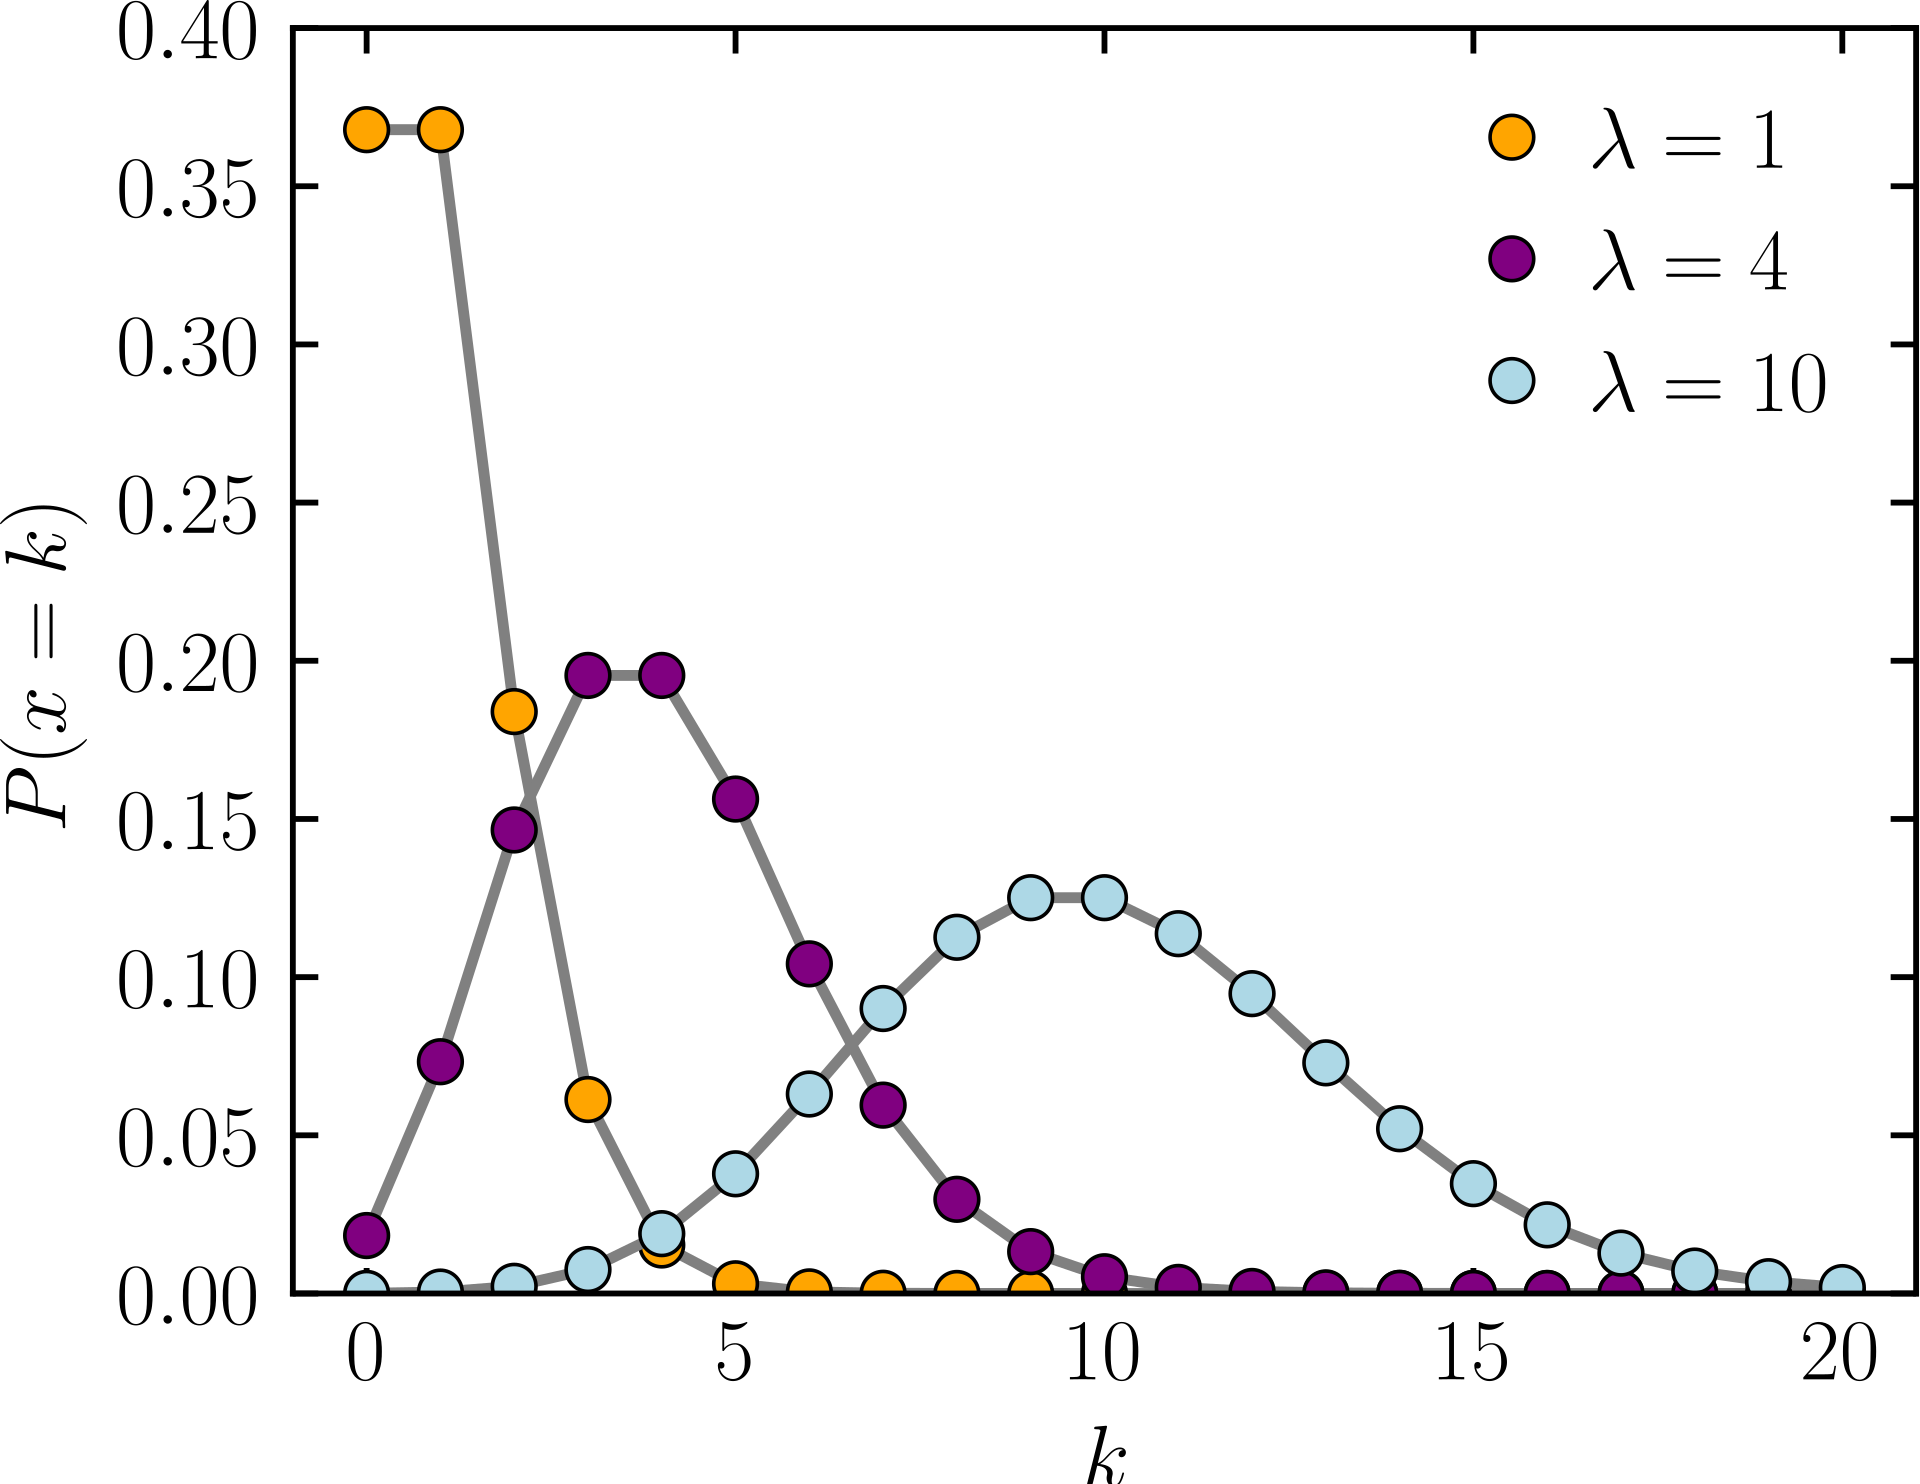
\includegraphics[scale=0.15]{img/Poisson_Distribution_Model.png}
\end{center}
It's CDF is: 
\begin{center}
    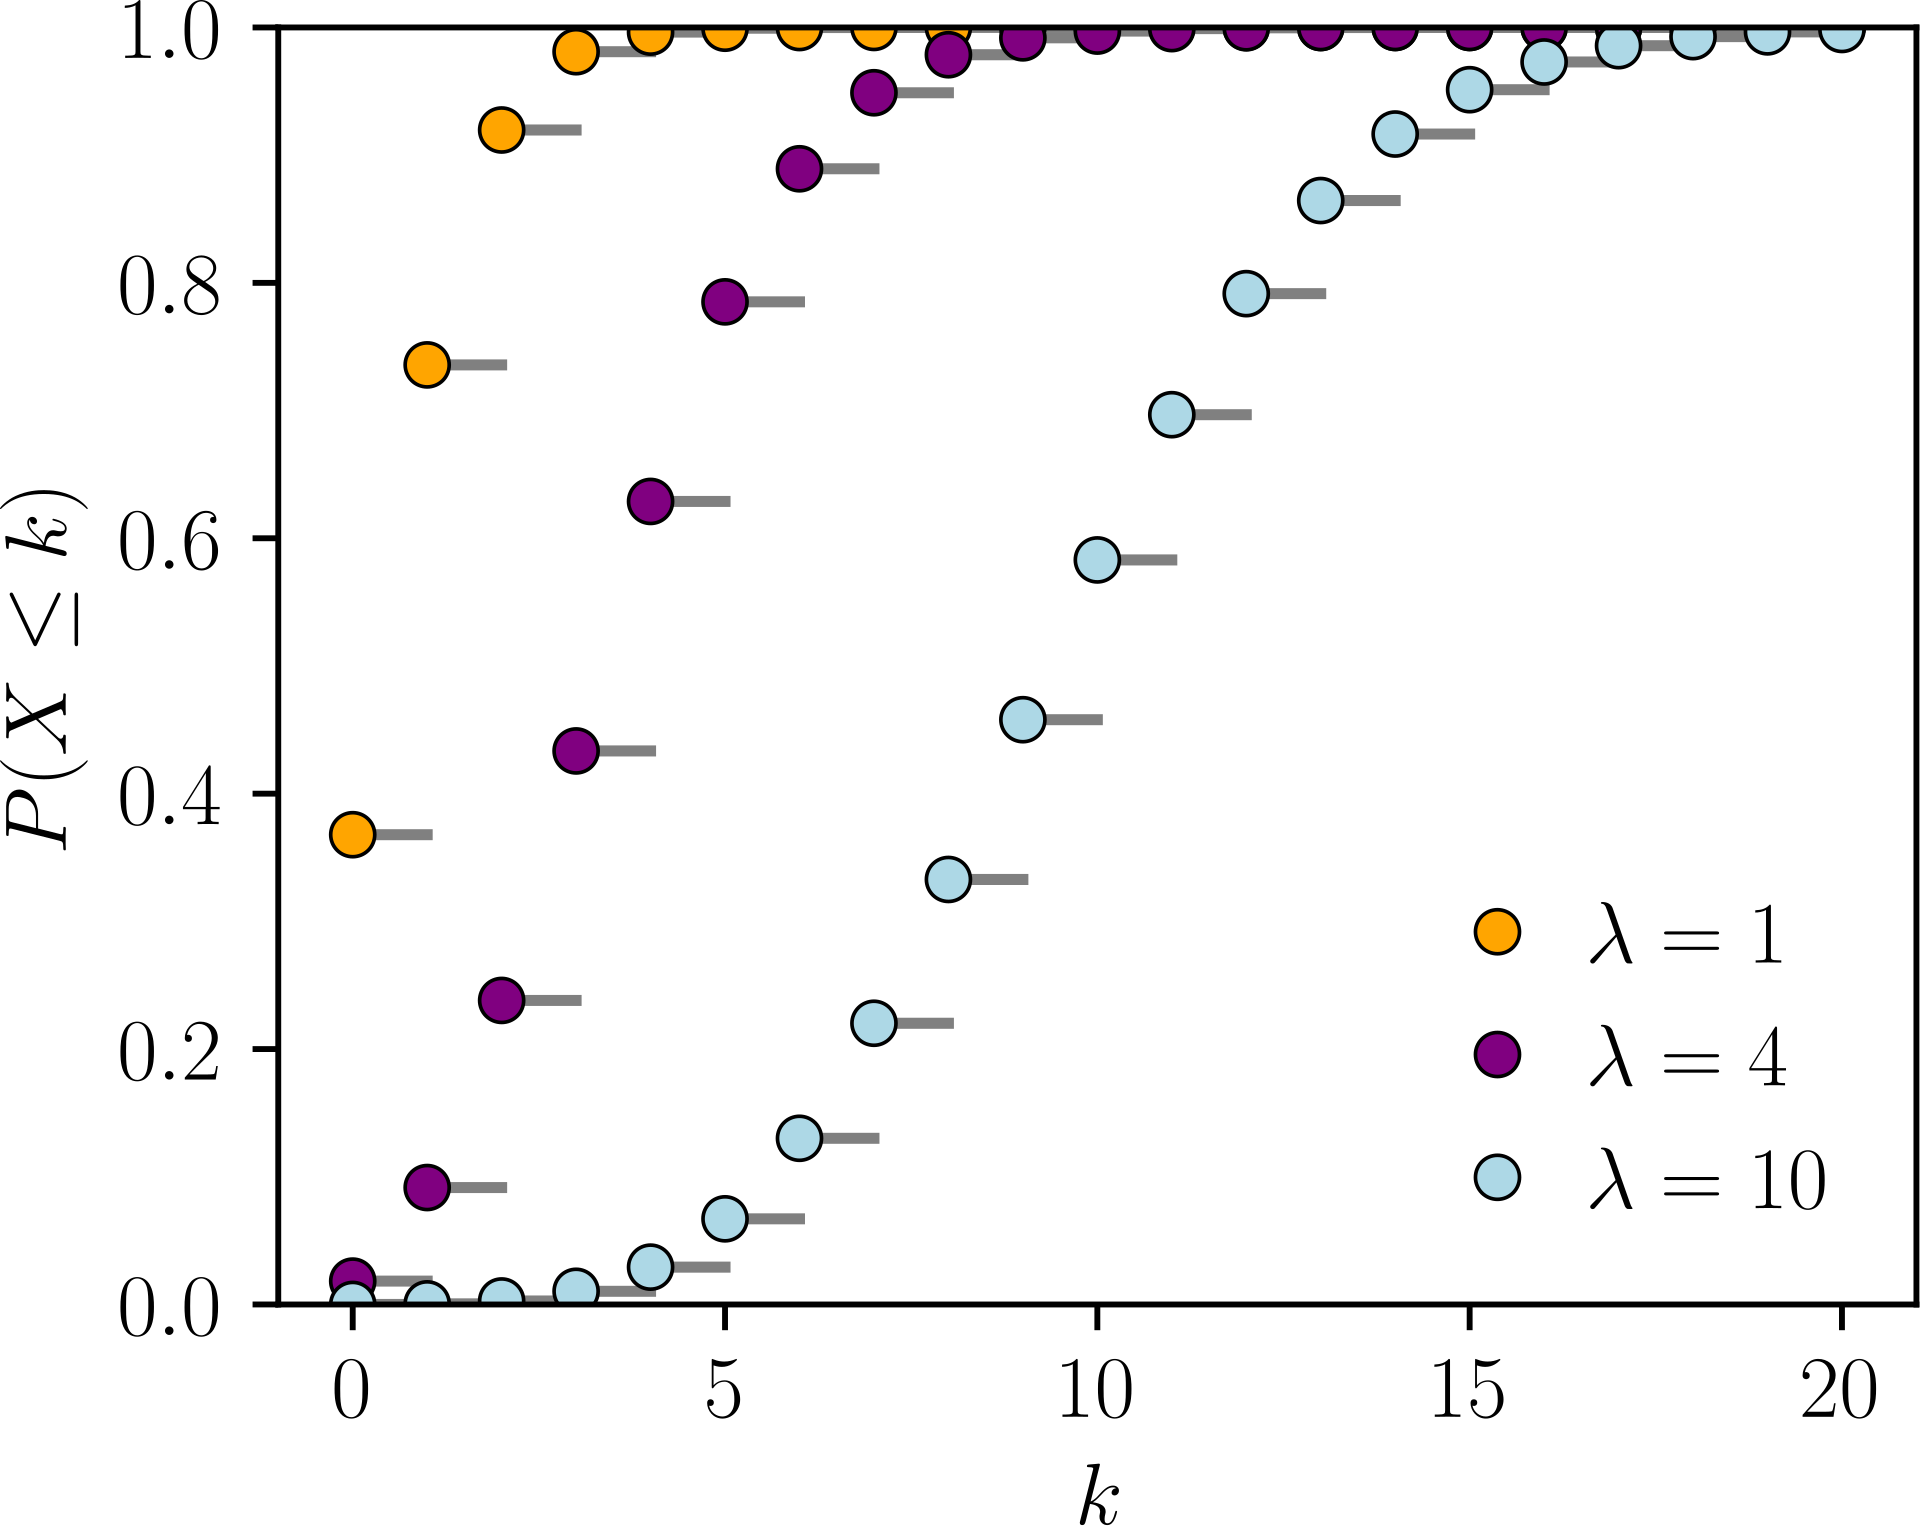
\includegraphics[scale=0.15]{img/Poisson_Distribution_Model_2.png}
\end{center}
\end{definition}

\begin{definition}[Negative Binomial Distribution]
The negative binomial distribution, denoted NB$(r, p)$ is defined as
\[\mathbb{P}(X = x) \equiv {{k+r-1} \choose k} \, (1-p)^r \, p^k\]
It can be interpreted as the distribution that models the number of successes in a sequence of iid Bernoulli-$p$ trials before a specified number $r$ failures occurs. 
\begin{center}
    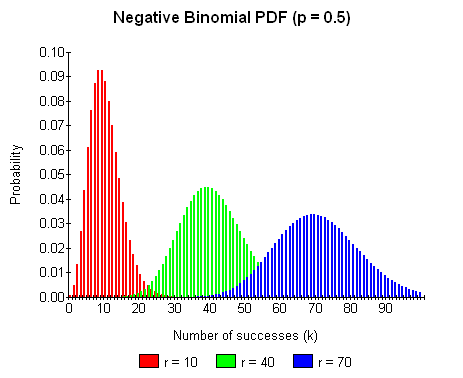
\includegraphics[scale=0.5]{img/Negative_Binomial_Distribution_Model.png}
\end{center}

\end{definition}

\subsection{Continuous Random Variables}
\begin{definition}
A real valued random variable $X$ is \textit{continuously distributed with density $f(x)$} if, for all $a < b$
\[\mathbb{P}(a \leq x \leq b) = \int_a^b f(x) \, dx\]
This continuous distribution is also called the \textit{probability density function} (PDF). Clearly, it must satisfy
\[f(x) \geq 0 \; \forall x \in \Omega \text{ and } \int_{\Omega} f(x)\, dx = \int_{-\infty}^\infty f(x) \, dx = 1\]
\end{definition}

\begin{definition}[Uniform]
A \textit{Uniform($a, b$)} distribution is defined 
\[f(x) = \begin{cases}
\frac{1}{|b-a|} & x \in [a, b] \\
0 & x \not\in [a,b]
\end{cases}\]
The CDF is defined
\[F(x) = \begin{cases}
0 & x < a \\
\frac{x-a}{b-a} & x \in [a, b] \\
1 & x > b
\end{cases}\]
\end{definition}

To introduce the CDF of the Normal distribution, we must first define the error function. 

\begin{definition}
The \textit{error function} is defined
\[erf (z) \equiv \frac{2}{\sqrt{\pi}} \int_0^z e^{-t^2} \, dt\]
This function is encountered when integrating the normal distribution. 
\end{definition}

\begin{definition}[Normal]
A \textit{Normal($\mu$, $\sigma^2$)} distribution is defined
\[f(x) = \frac{1}{\sqrt{2 \pi \sigma^2}} e^{-\frac{(x-\mu)^2}{2\sigma^2}}, \; x \in \mathbb{R}\]
\begin{center}
    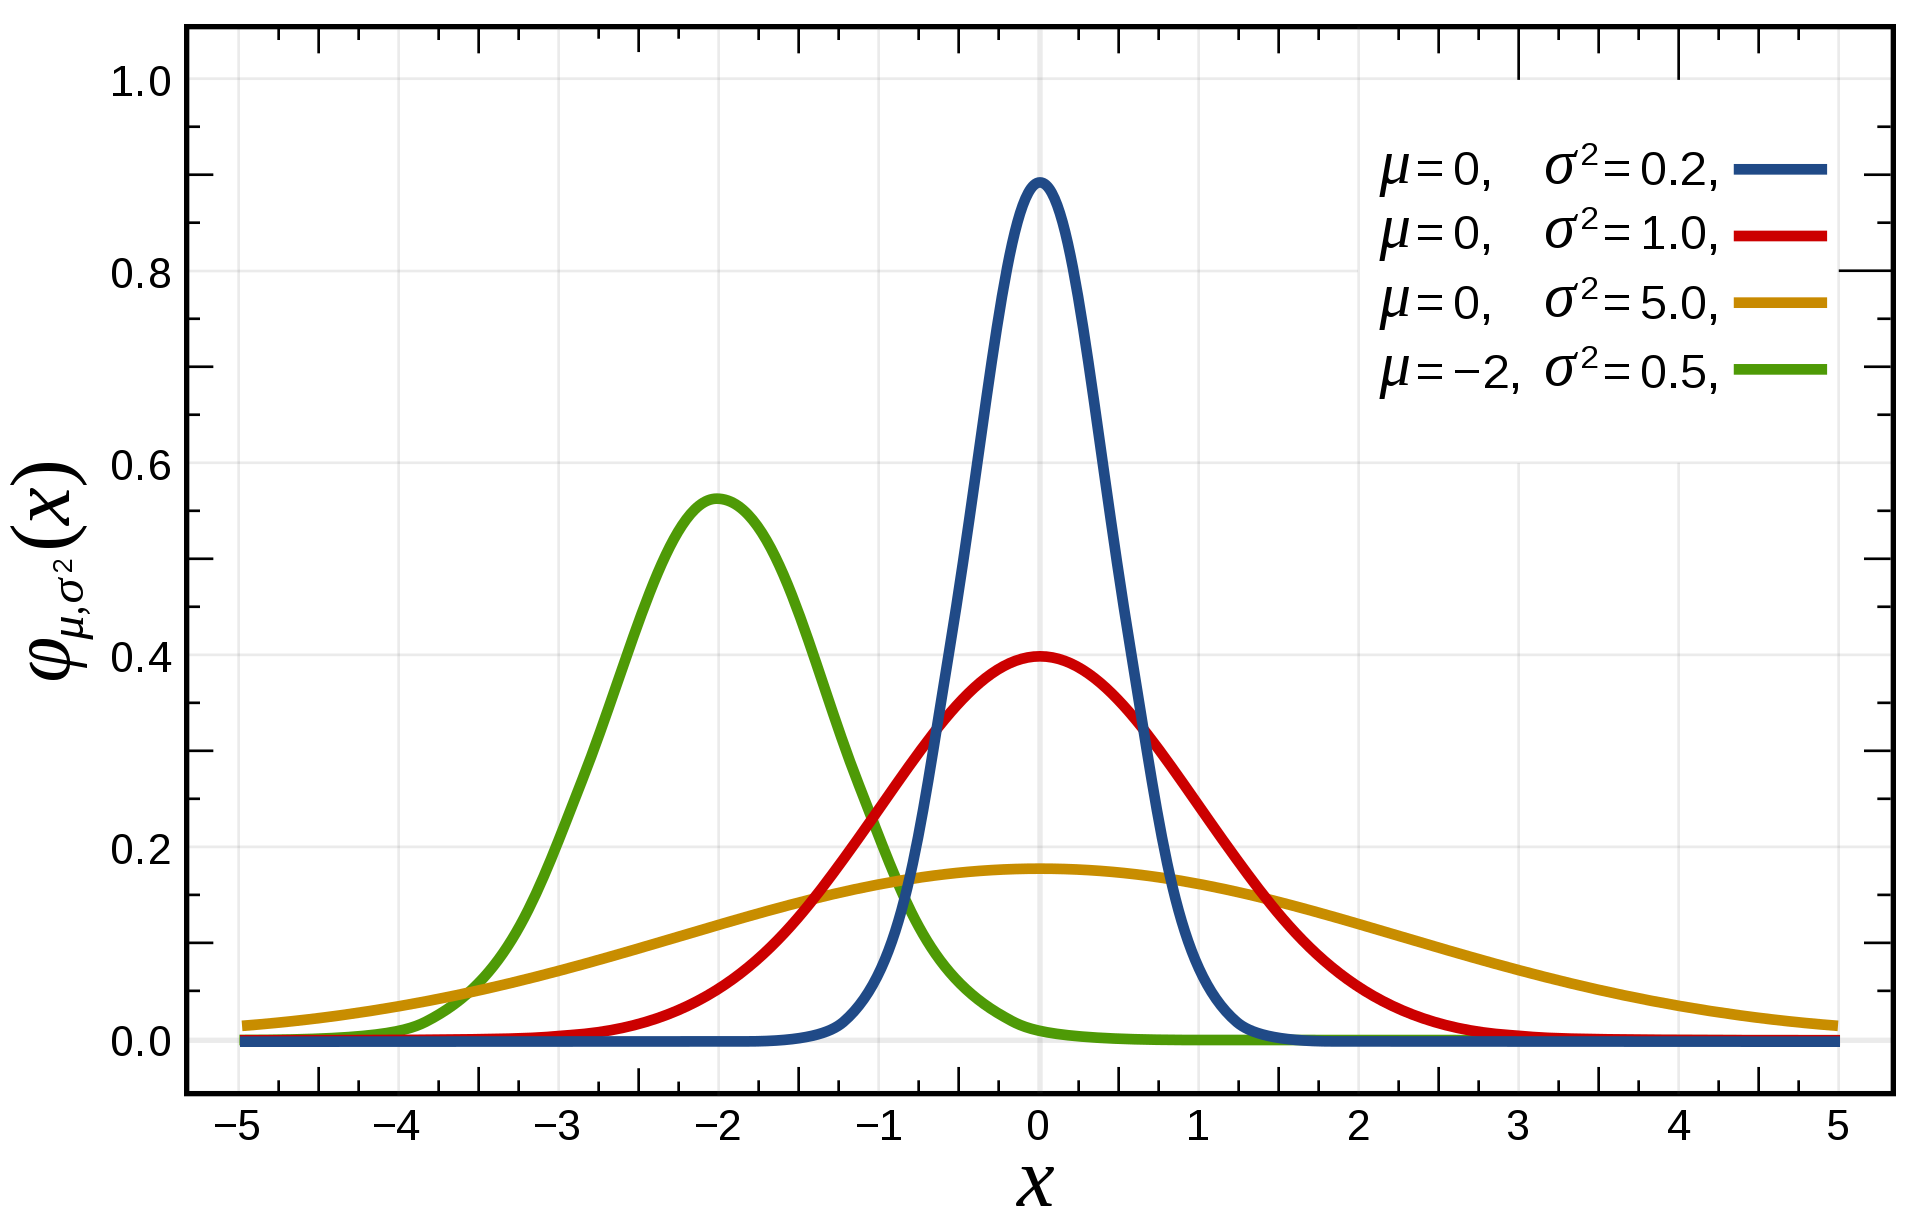
\includegraphics[scale=0.15]{img/Normal_Distribution_Model.png}
\end{center}
It is worthwhile to remember the standardized normal distribution Normal($0$, $1$).
\[f(x) = \frac{1}{\sqrt{2\pi}} e^{-\frac{x^2}{2}}, \; x \in \mathbb{R}\]
It's CDF is computed with usual integration, but for the sake of consistency, we provide a formula. 
\[F(x) = \frac{1}{2} \bigg(1 + erf\Big(\frac{x-\mu}{\sigma \sqrt{2}}\Big) \bigg)\]
\begin{center}
    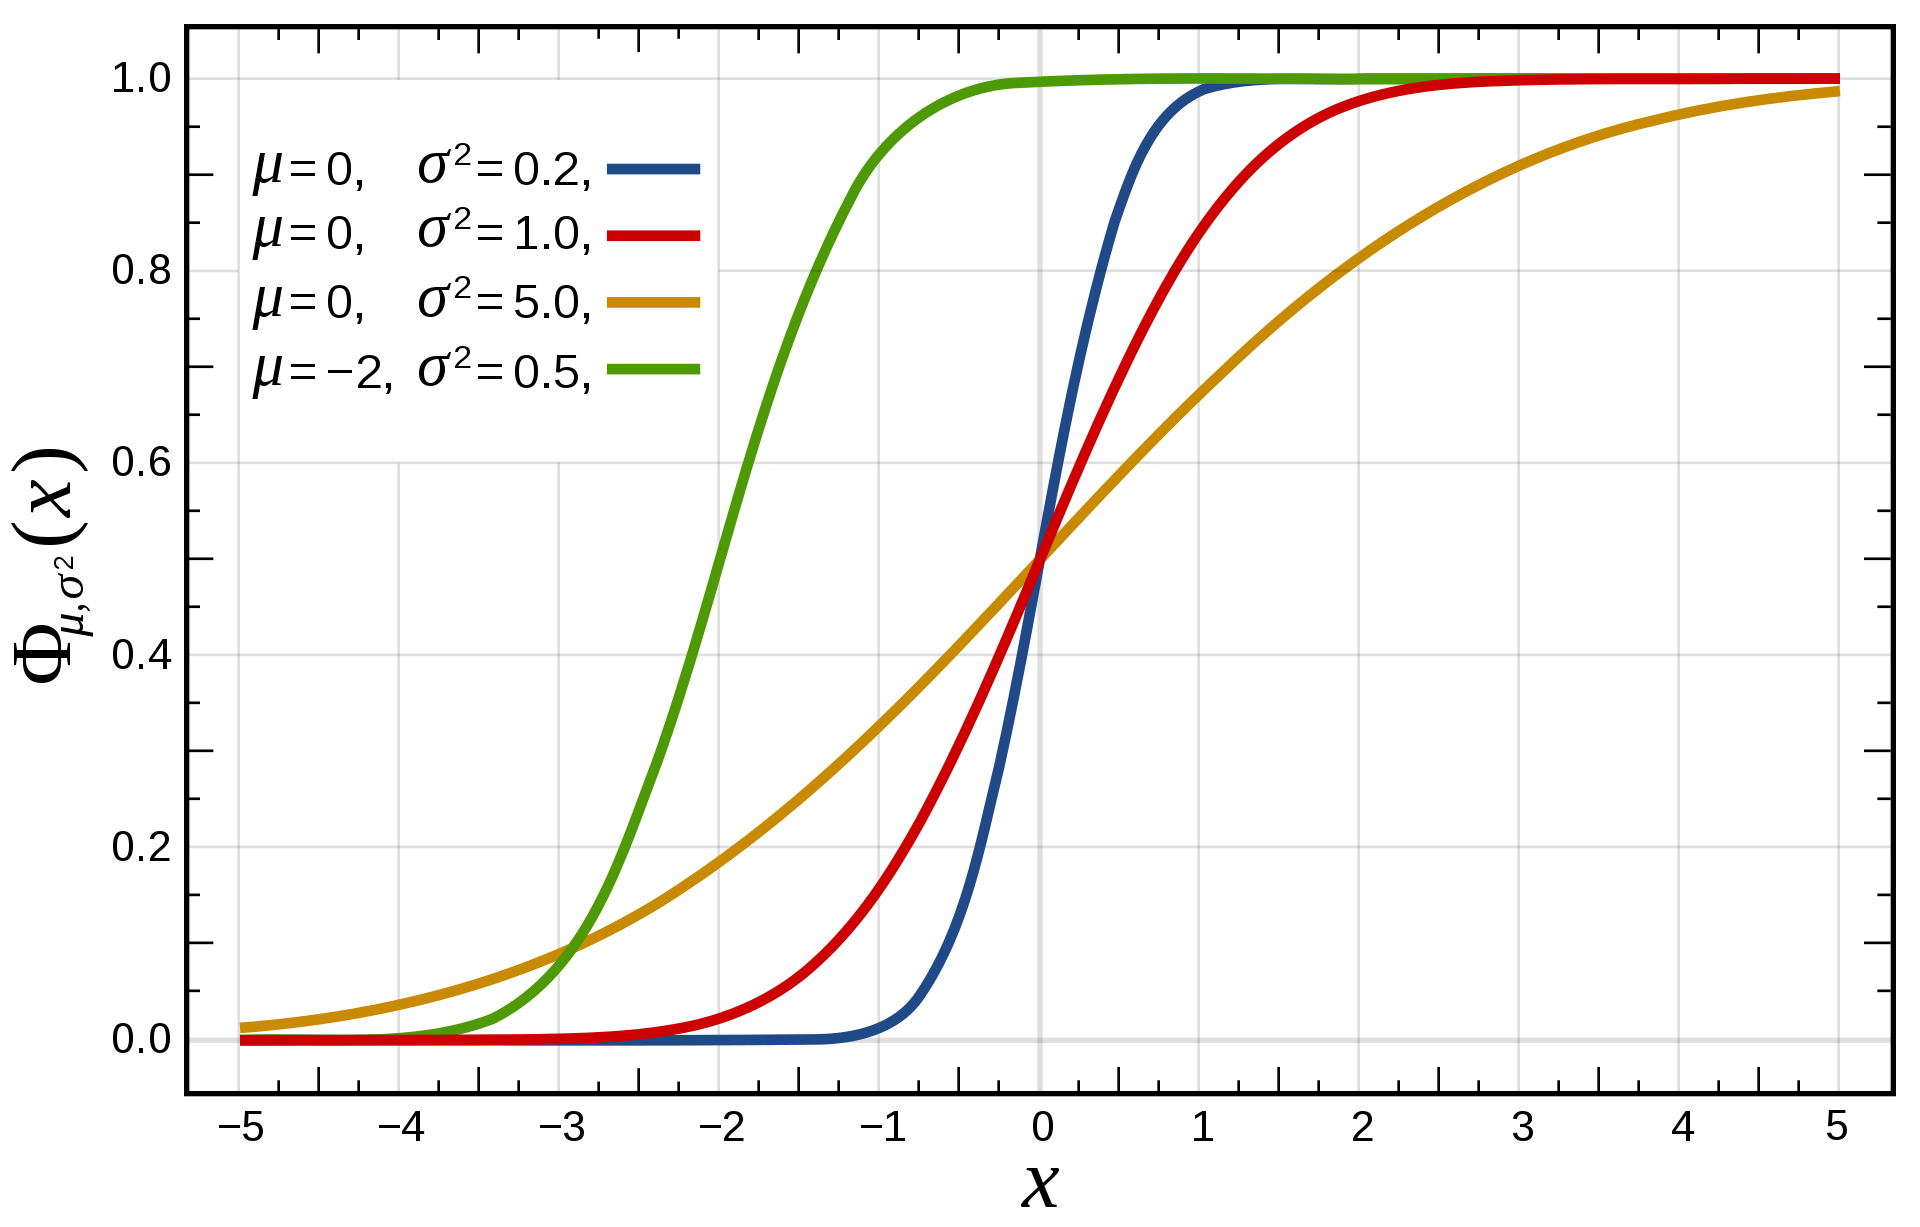
\includegraphics[scale=0.15]{img/Normal_Distribution_Model_2.png}
\end{center}
\end{definition}

\begin{definition}[Exponential]
A \textit{Exponential($\lambda$)} distribution is defined
\[f(x) = \begin{cases}
\lambda e^{-\lambda x} & x \geq 0 \\
0 & x < 0
\end{cases}\]
\begin{center}
    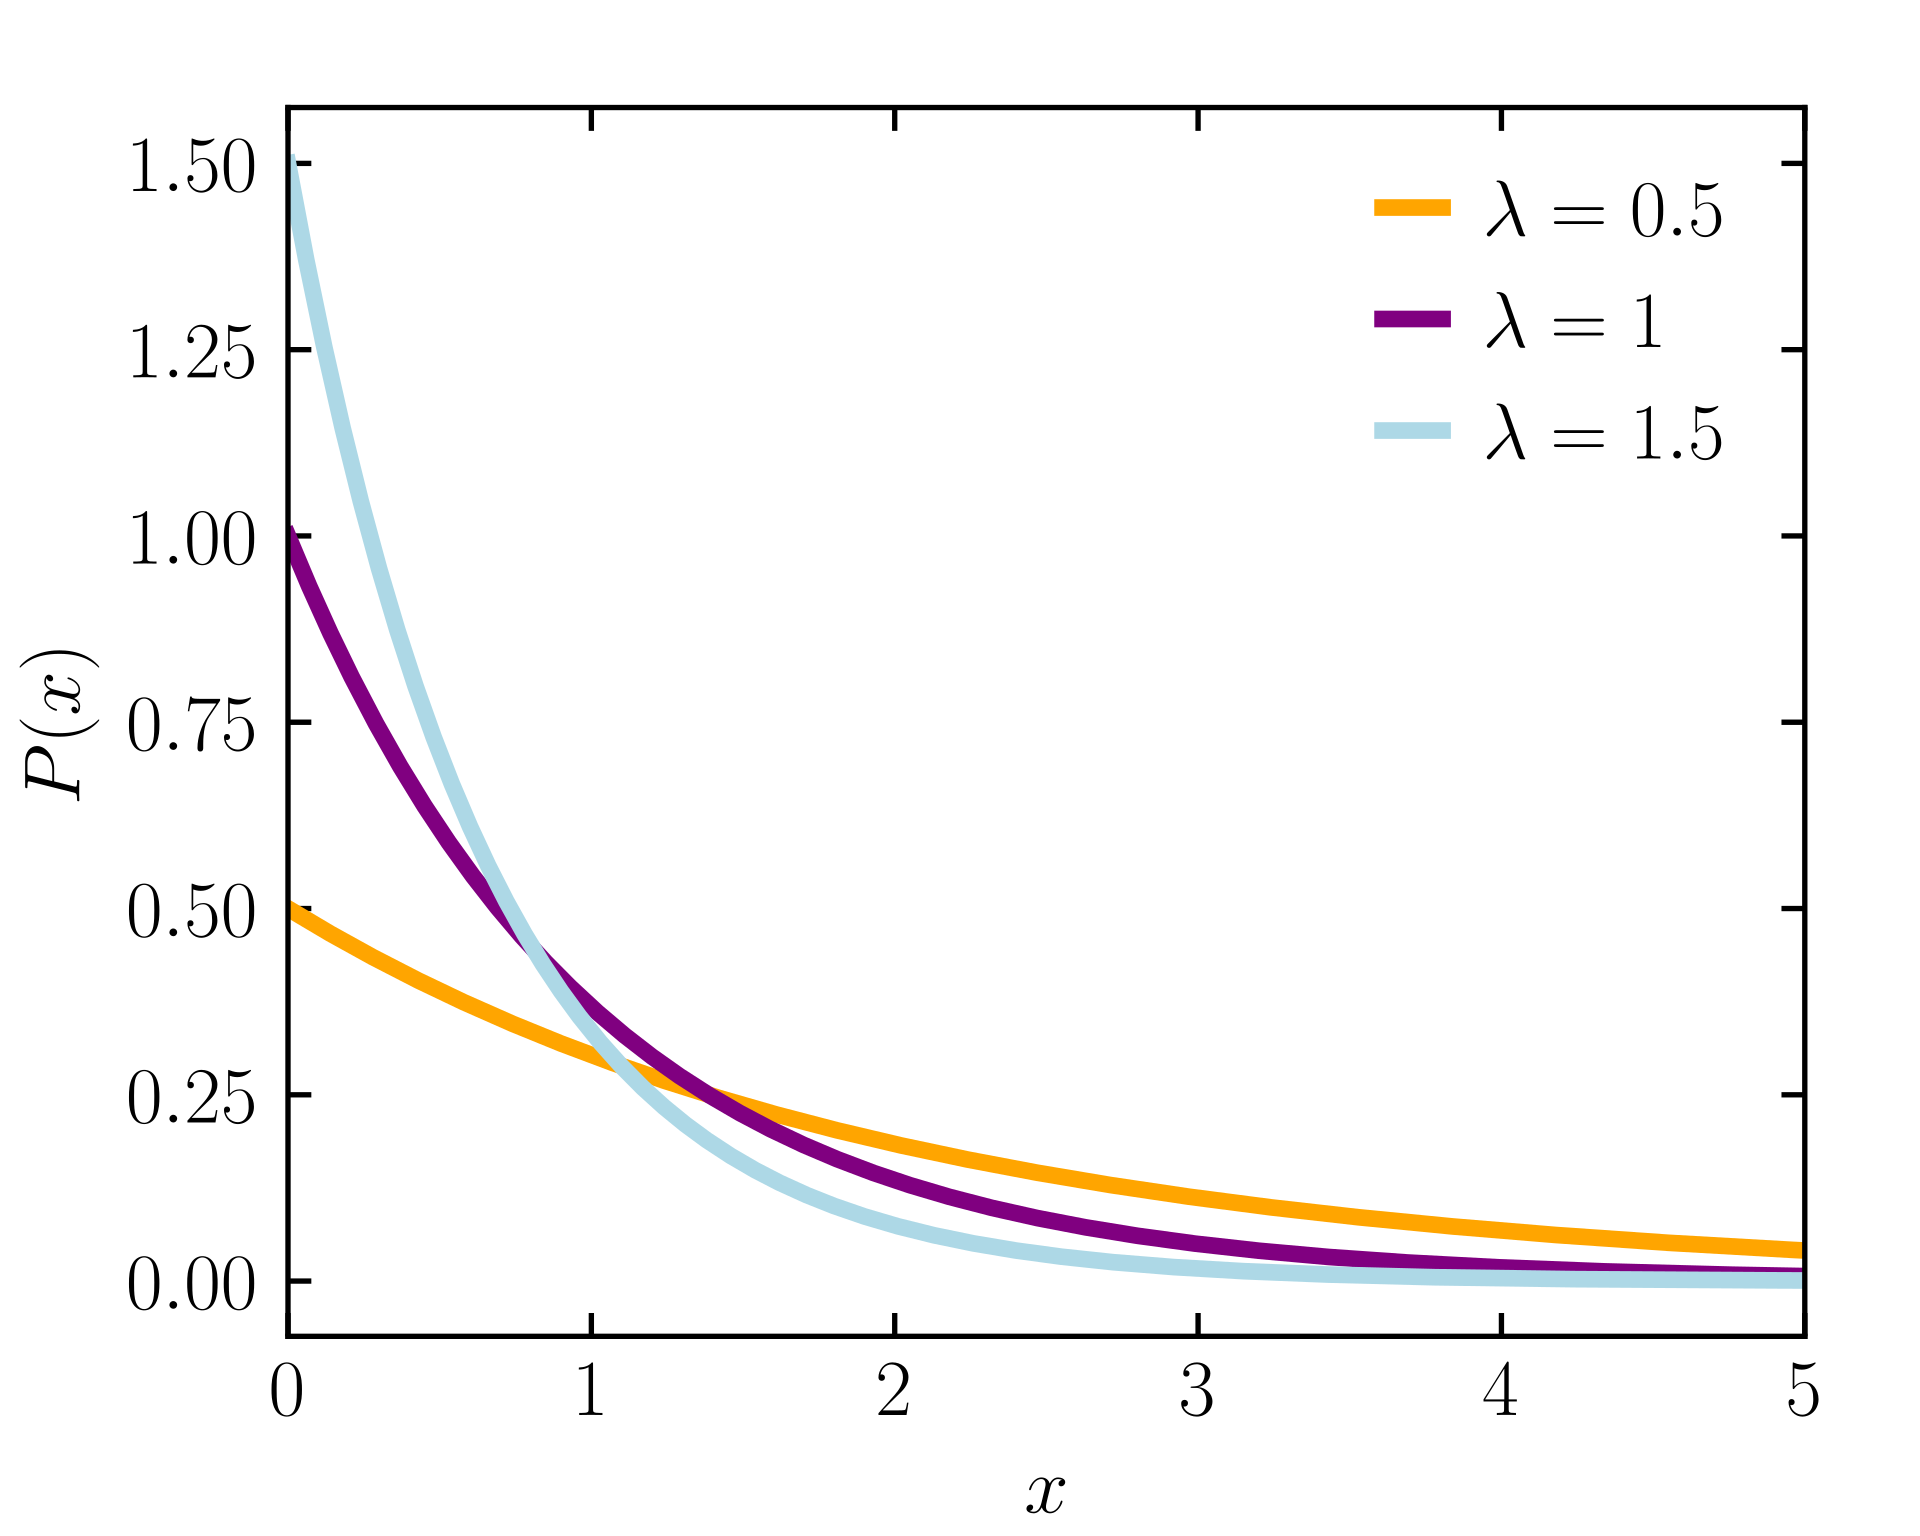
\includegraphics[scale=0.15]{img/Exponential_Distribution_Model.png}
\end{center}
The CDF is defined
\[F(x) = 1 - e^{-\lambda x}\]
\begin{center}
    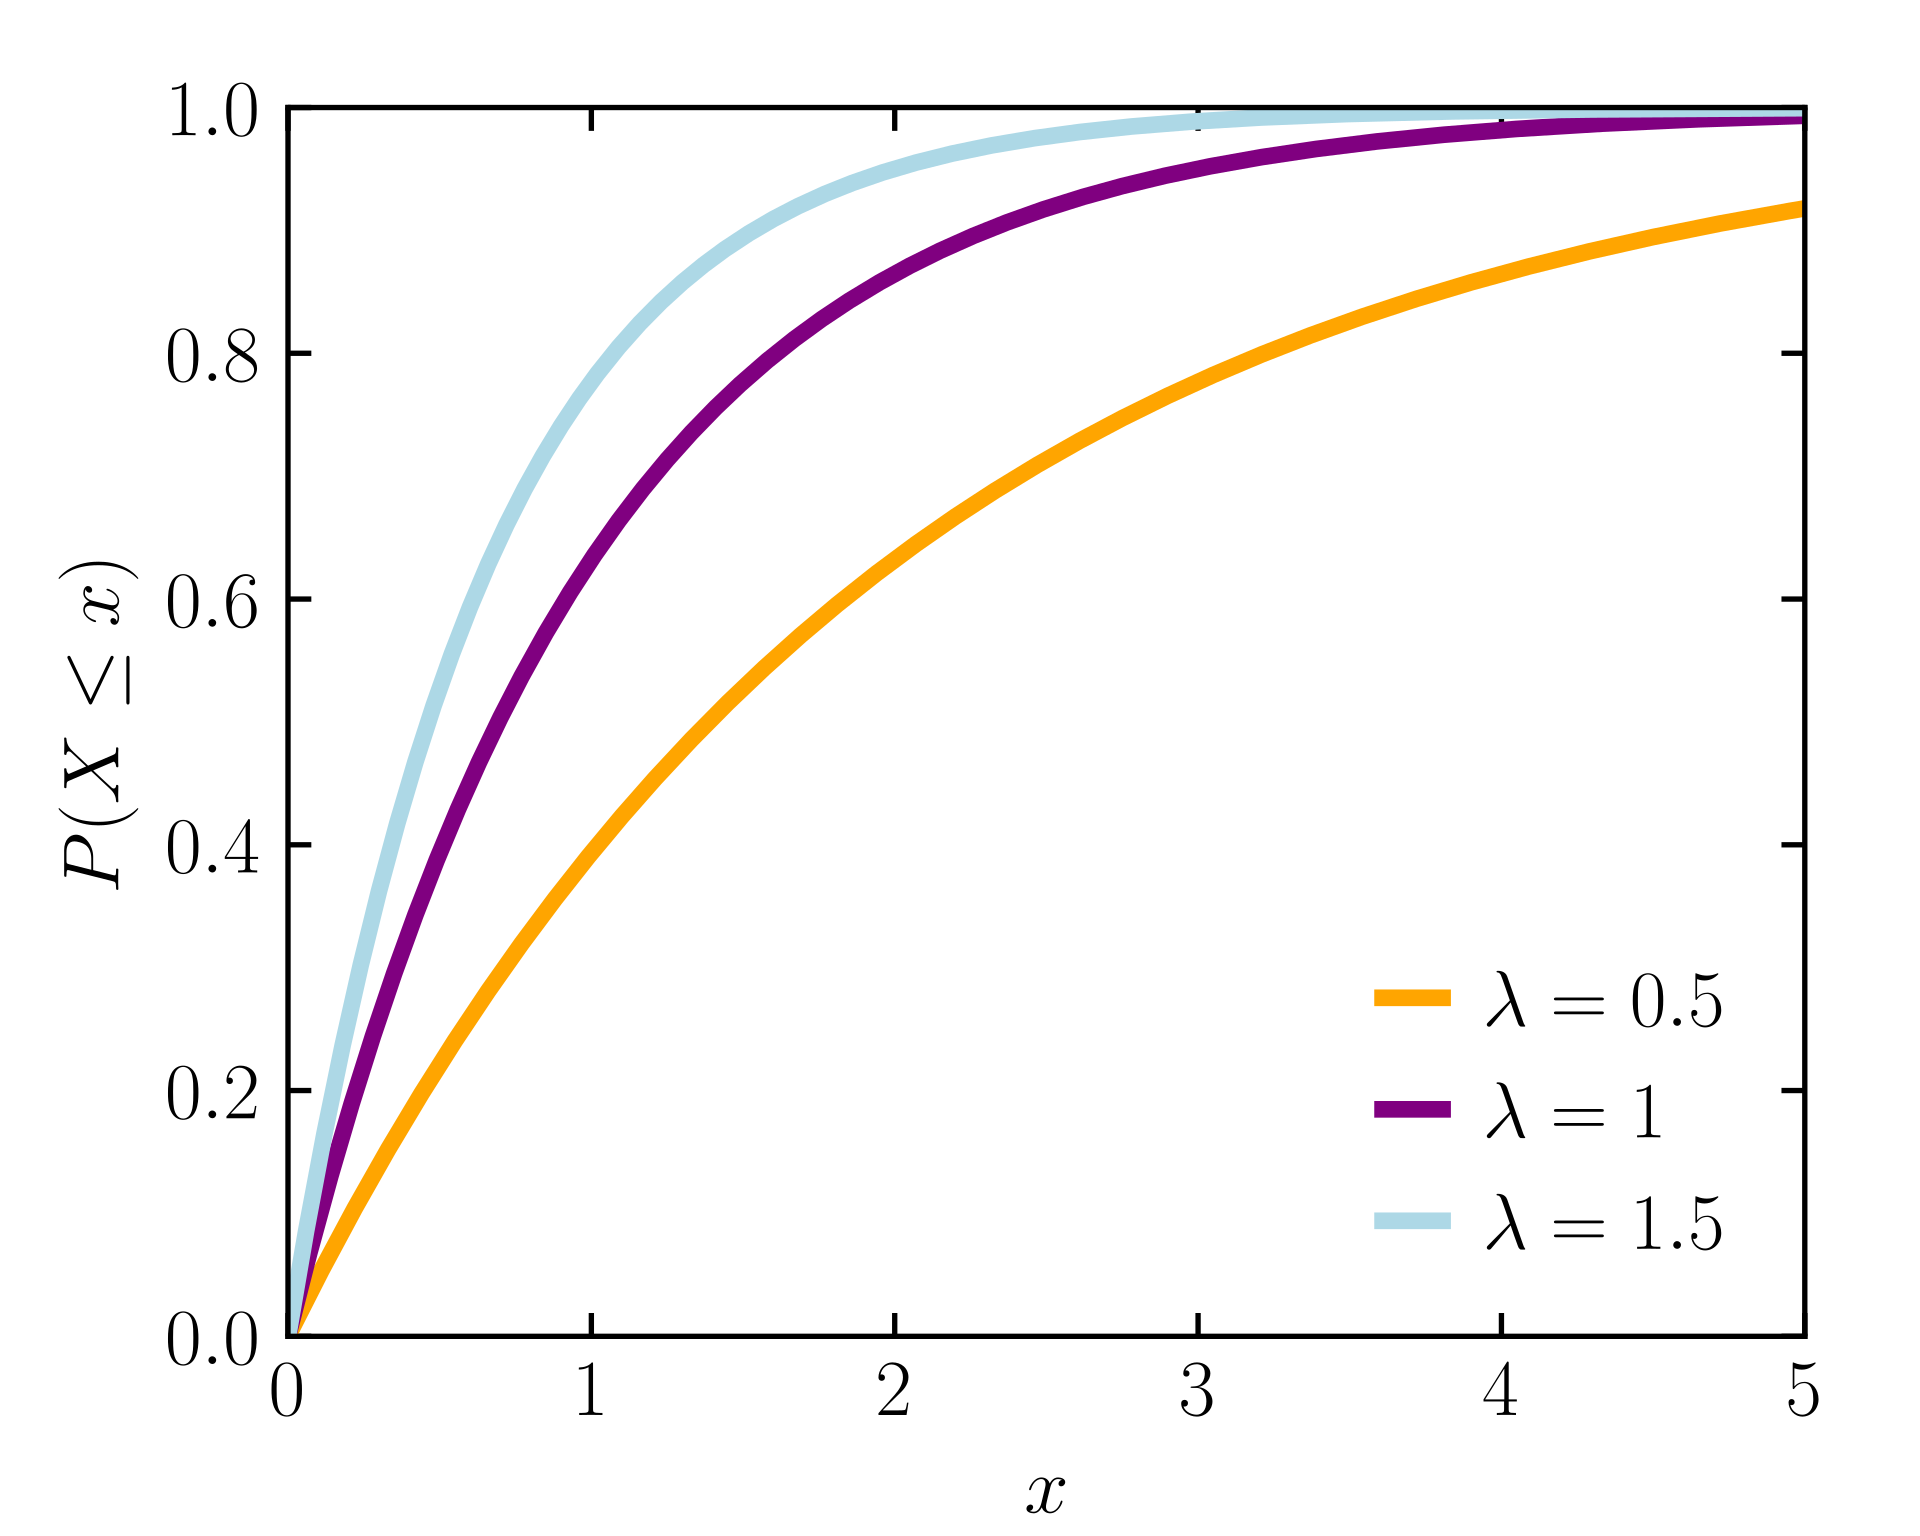
\includegraphics[scale=0.15]{img/Exponential_Distribution_Model_2.png}
\end{center}
Notice the similarity between an exponential distribution (continuous) and a geometric distribution (discrete). 
\end{definition}

\begin{definition}[Gamma Function]
The \textit{Gamma function} is a commonly used function used extension of the factorial function to the complex numbers. It can be interpreted as a solution to the problem: \textit{Find a smooth curve that connects the points $(x, y)$ given by $y = (x-1)!$ at the positive integer values for $x$.} That is, for any positive integer $x$, 
\[\Gamma(x) \equiv (x-1)!\]
The extension of this for complex numbers with a positive real part is defined with an improper convergent integral: 
\[\Gamma(z) \equiv \int_{0}^\infty x^{z-1} e^{-x}\, dx, \;\;\;\;\; \text{Re}(z) > 0\]
The gamma function is then defined as the analytic continuation of the integral function to the rest of the complex numbers. 
\end{definition}

\begin{definition}[Gamma]
A \textit{Gamma($n$, $\lambda$)}, or with different notational parameters, Gamma($n$, $\theta = 1/\lambda$) distribution for natural numbers $n$ is defined 
\[f(x) = \frac{\lambda^n x^{n-1}}{(n-1)!} e^{-\lambda x} = \frac{x^{n-1}}{\theta^n (n-1)!} e^{-x/\theta}, \;\;\; x \geq 0\]
but the general case for all $n \in \mathbb{R}$ results in the factorial being replaced by the Gamma function: 
\[f(x) = \frac{\lambda^n x^{n-1}}{\Gamma(n)} e^{-\lambda x} = \frac{x^{n-1}}{\theta^n \Gamma(n)} e^{-x/\theta}\;\;\; x \geq 0\]
\begin{center}
    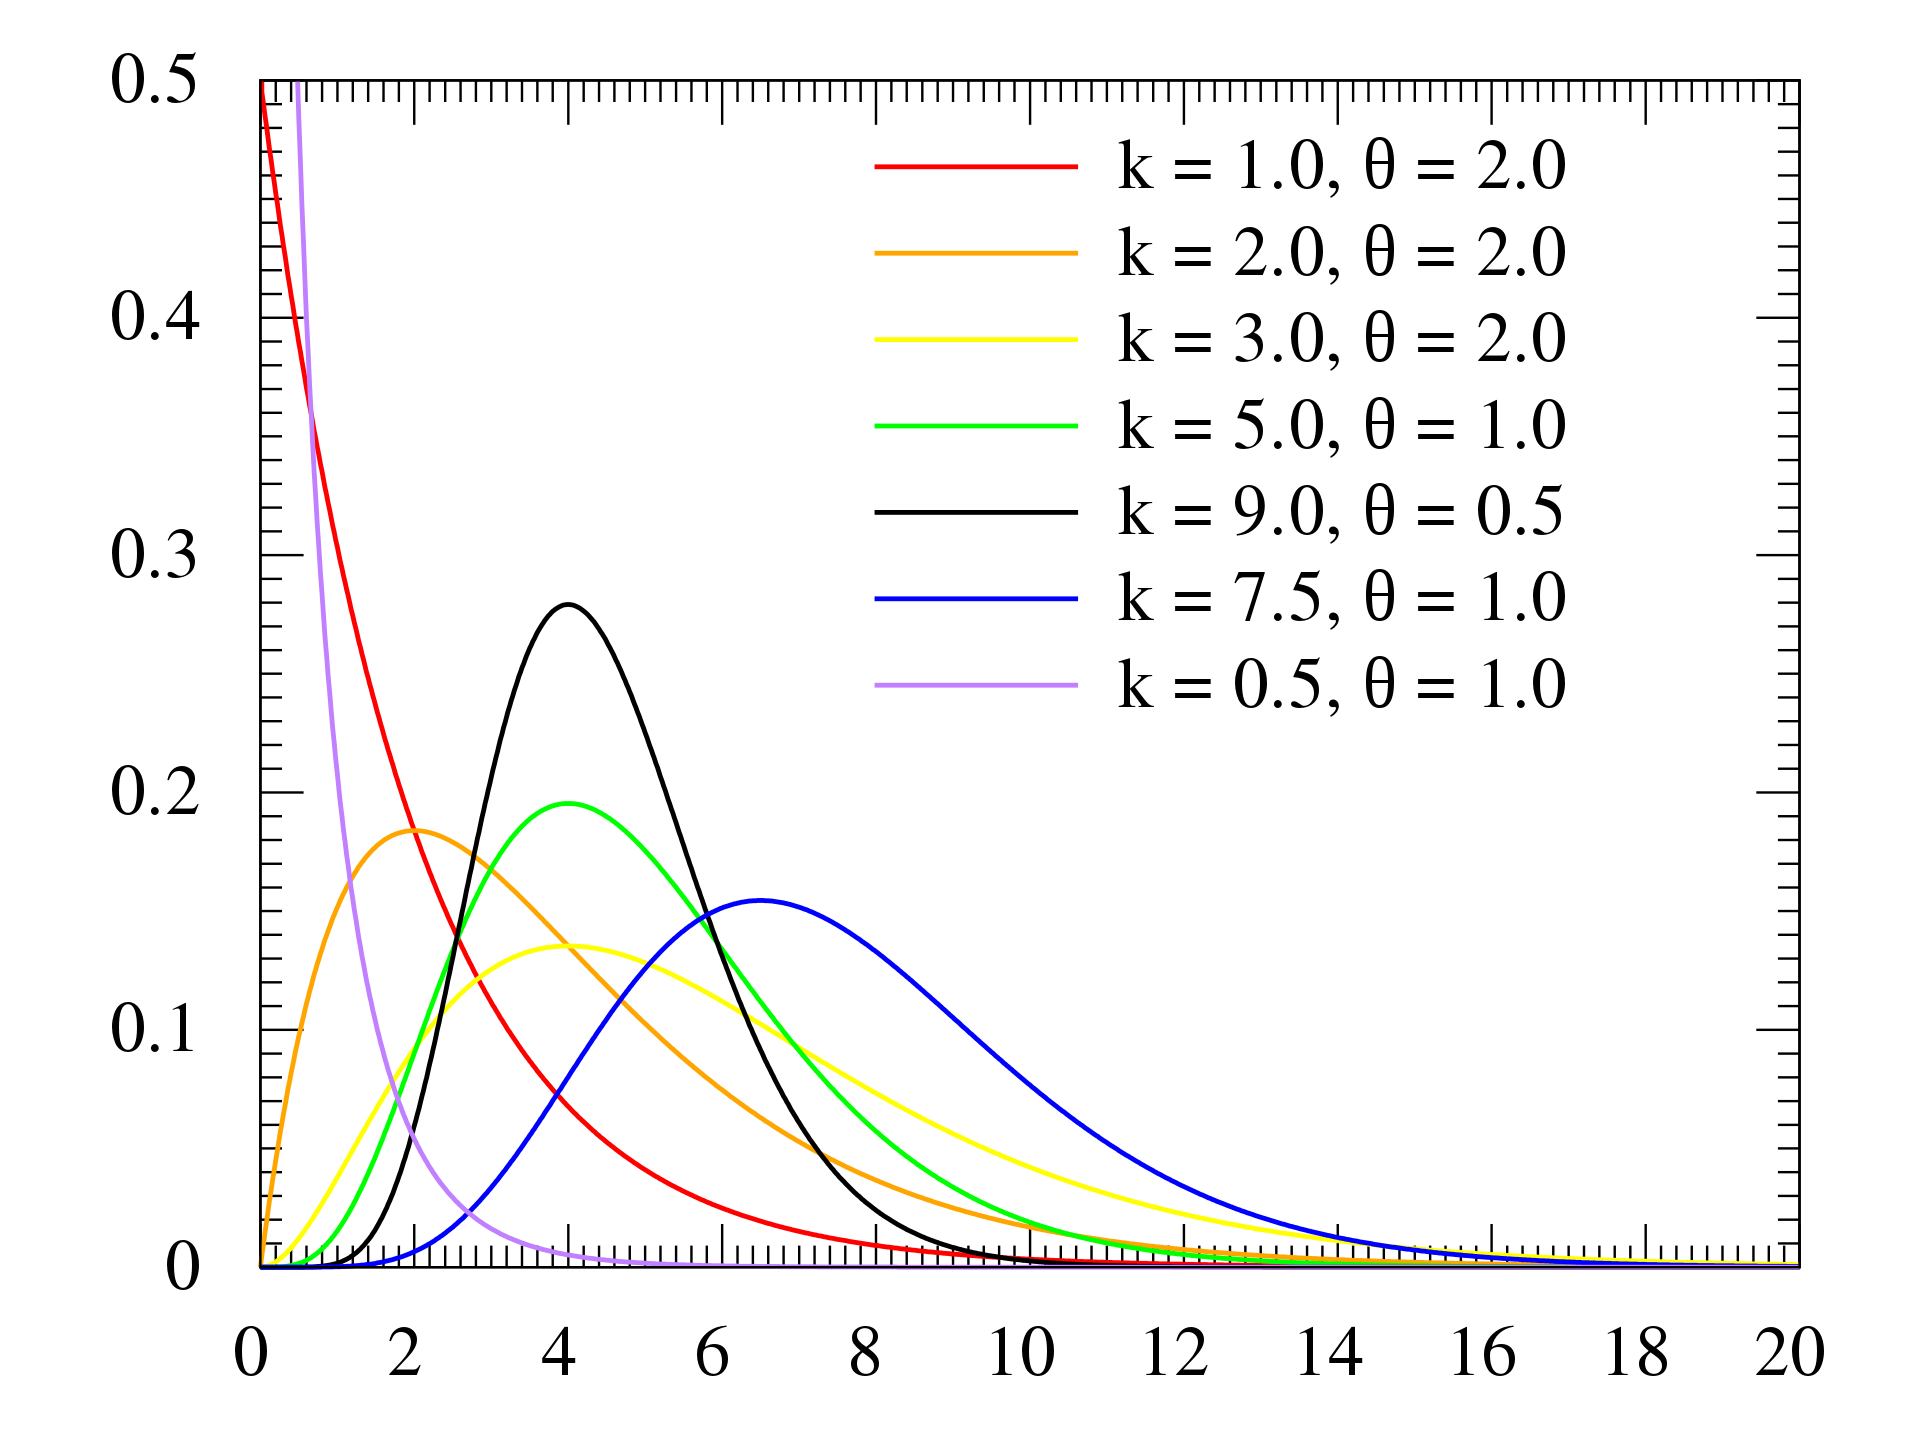
\includegraphics[scale=0.15]{img/Gamma_Distribution_Model.png}
\end{center}
Note that Gamma(1, $\lambda$) is precisely the exponential density Exp($\lambda$). Its CDF is: 
\begin{center}
    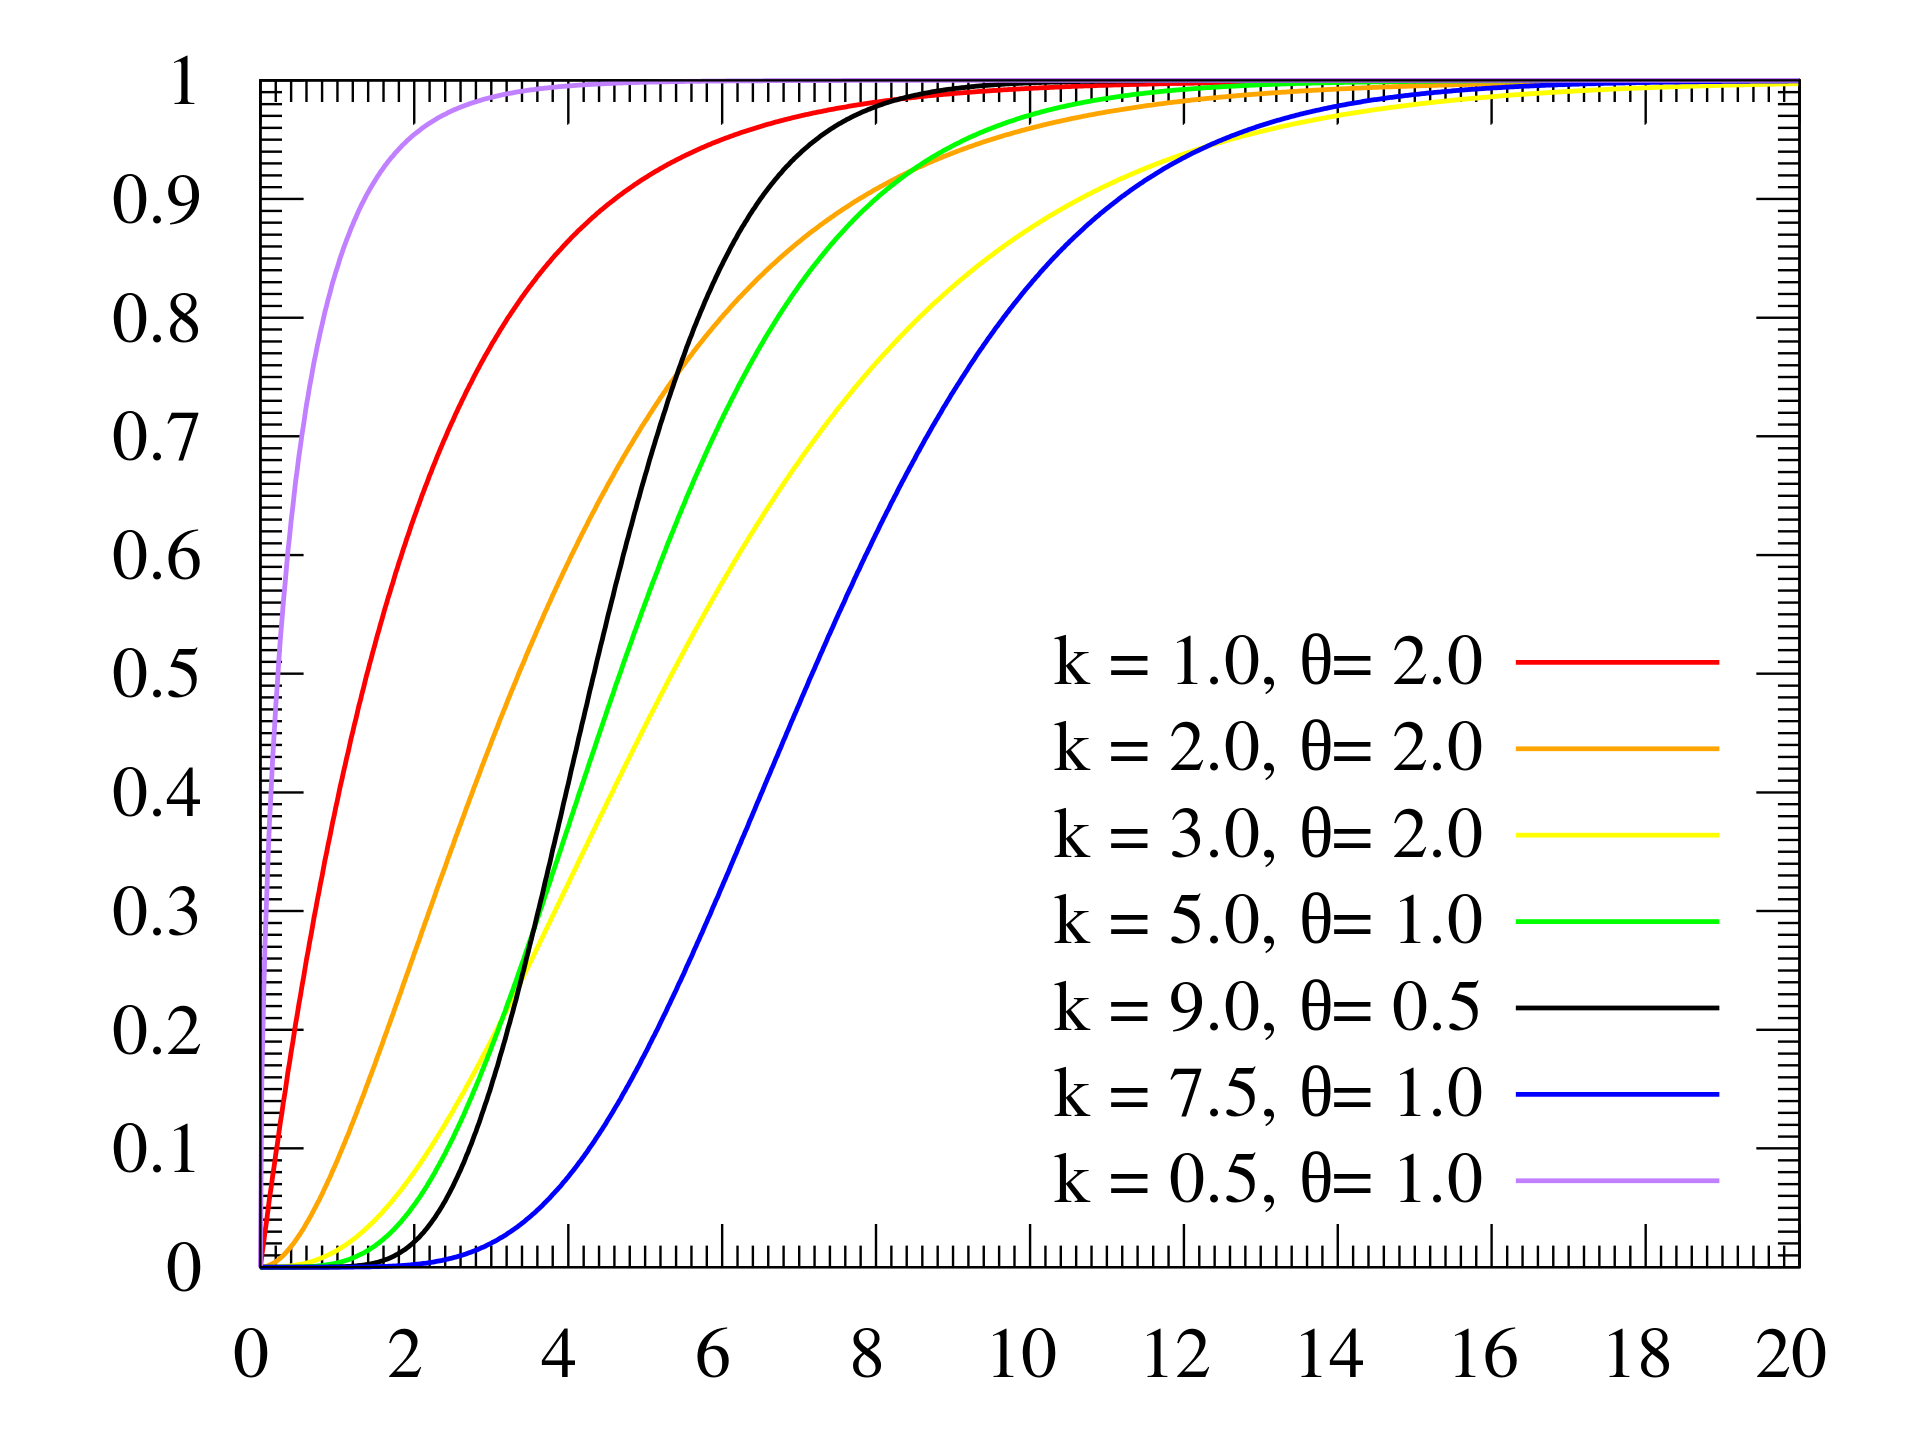
\includegraphics[scale=0.15]{img/Gamma_Distribution_Model_2.png}
\end{center}
\end{definition}

\begin{definition}[Beta Distribution]
A \textit{Beta($\alpha$, $\beta$)} distribution for positive real numbers $\alpha, \beta$ is defined
\[f(x) \equiv \frac{x^{\alpha-1} \,(1-x)^{\beta-1}}{B(\alpha, \beta)}, \text{ where } B(\alpha, \beta) \equiv \frac{\Gamma(\alpha) \Gamma(\beta)}{\Gamma(\alpha + \beta)}\]
and $\Gamma$ is the Gamma function. 
\begin{center}
    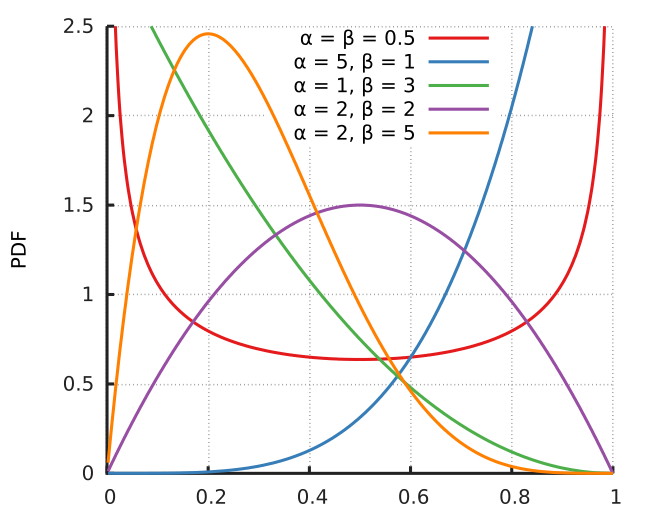
\includegraphics[scale=0.4]{img/Beta_Distribution_Model.png}
\end{center}
Its CDF is
\begin{center}
    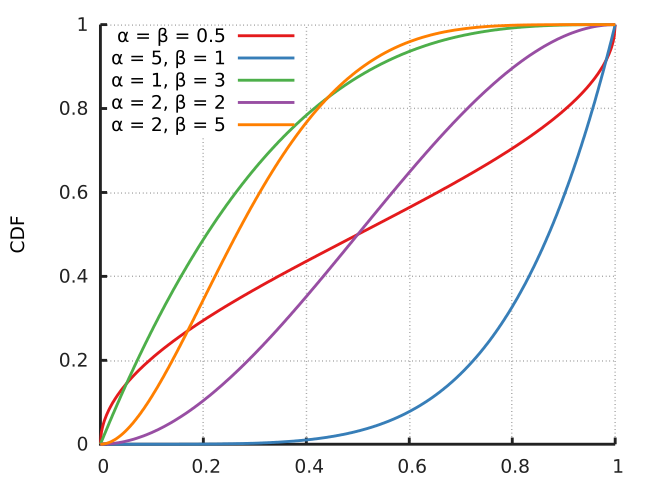
\includegraphics[scale=0.4]{img/Beta_Distribution_Model_2.png}
\end{center}
The generalization of the Beta distribution to multiple variables is called the \textit{Dirichlet distribution}. 
\end{definition}

\section{Expectation, Variance} 
\begin{definition}
The expectation of a discrete random variable $X: \Omega \longrightarrow \mathbb{R}$ is 
\[\mathbb{E}(X) = \sum_{x \in \im(X)} x \, \mathbb{P}(X = x)\]
where the sum is over the countable set of all possible values of $X$, assuming that the sum converges absolutely. 
\end{definition}

\begin{definition}
The expectation of a continuous random variable $X$ with density $f(x)$ is the integral 
\[\int_\mathbb{R} x \, f(x) \, dx\]
assuming that the integral converges absolutely. 
\end{definition}

It is possible that the expectation is infinite or not well-defined. In any case, the expectation is a property of the distribution. If two random variables have the same distribution, then $\mathbb{E}(X) = \mathbb{E}(Y)$. We now state some properties of expectation. 

\begin{proposition}
Expectation is a linear operator from the space of all discrete distributions to $\mathbb{R}$. That is, for any constants $\alpha, \beta \in \mathbb{R}$ and random variables $X, Y$ on $\Omega$, 
    \[\mathbb{E}(\alpha X + \beta Y) = \alpha \mathbb{E}(X) + \beta \mathbb{E}(Y)\] 
\end{proposition}
\begin{proof}
Let $V_X, V_Y \subset \mathbb{R}$ denote the ranges of $X$ and $Y$, respectively. That is, 
\[V_X \equiv \{x \in \mathbb{R} \; | \; \mathbb{P}(X =x) >0\}, \; V_Y \equiv \{y \in \mathbb{R} \; | \; \mathbb{P}(Y =y) > 0\}\]
Now, let $V_{X+Y}$ be the range of $X+Y$, explicitly defined
\[V_{X+Y} \equiv \{x+y \; | \; x \in V_X, y \in V_Y\}\]
Note that $V_X, V_Y$, and $V_{X+Y}$ are all countable sets. Then, we can define $\mathbb{E}(X+Y)$ through the joint distribution of $X$ and $Y$, and get
\begin{align*}
    \mathbb{E}(X+Y) & = \sum_{(x,y) \in V_{X+Y}} (x+y) \mathbb{P} (X=x, Y=y) \\
    & = \sum_{x \in V_X} \sum_{y \in V_Y} (x+y) \mathbb{P} (X=x, Y=y) \\
    & = \sum_{x \in V_X} x \sum_{y \in V_Y} \mathbb{P} (X=x, Y=y) + \sum_{y \in V_Y} y \sum_{x \in V_X} \mathbb{P} (X=x, Y=y) \\
    & = \sum_{x \in V_X} x \mathbb{P}(X=x) + \sum_{y \in V_Y} \mathbb{P}(Y=y) \\
    & = \mathbb{E}(X) + \mathbb{E}(Y)
\end{align*}
Proving linearity for scalar multiples is trivial, and will not be shown here. 
\end{proof}

\begin{theorem}[Expectations of functions]
Given a function $g: \mathbb{R} \longrightarrow \mathbb{R}$, 
\[\mathbb{E} \big( g(X) \big) = \sum_x g(x) \, \mathbb{P}(X = x)\]
in the discrete case. If $X$ has density $f$, then 
\[\mathbb{E} \big( g(X) \big) = \int_\mathbb{R} g(x) \, f(x) \, dx\]
For multivariate functions $g: \mathbb{R} \times \mathbb{R} \longrightarrow \mathbb{R}$ in joint distributions, we have
\[\mathbb{E}\big( g(X, Y) \big) = \sum_{x, y} g(x, y) \, \mathbb{P} (X=x, Y=y)\]
\end{theorem}

\begin{proposition}[Expectation of Independent Events]
If $X$ and $Y$ are independent random variables, 
\[\mathbb{E}(XY) = \mathbb{E}(X) \, \mathbb{E}(Y)\]
\end{proposition}

\begin{theorem}[Tail Sum Formula]
If a discrete random variable $X$ takes values in the non-negative integers $\{0, 1, 2, 3, ...\}$, then 
\[\mathbb{E}(X) = \sum_{k=1}^\infty \mathbb{P}(X \geq k)\]
In any case (continuous or discrete), if $X$ is a non-negative random variable, then 
\[\mathbb{E}(X) = \int_0^\infty \mathbb{P}(X > x) \, dx = \int_0^\infty 1 - F(x) \, dx\]
where $F$ is the CDF of $X$. 
\end{theorem}
\begin{proof}
Suppose that $X$ takes values in $\{0, 1, 2, 3, ...\}$. Then, 
\begin{align*}
    \mathbb{E}(X) & = \sum_{k \geq 1} k \, \mathbb{P}(X=k) \\
    & = \sum_{k\geq 1} \sum_{j=1}^k \mathbb{P}(X = k) \\
    & = \sum_{k \geq 1} \sum_{j=1}^k \mathbb{I}_{j \leq k} \, \mathbb{P}(X=k) \\
    & = \sum_{j=1}^\infty \sum_{k \geq 1} \mathbb{I}_{j \leq k} \, \mathbb{P}(X =k) \\
    & = \sum_{j=1}^\infty \sum_{k \geq j} \mathbb{P}(X=k) \\
    & = \sum_{j=1}^\infty \mathbb{P}(X \geq j)
\end{align*}
\end{proof}

We can actually use linear algebra to optimize approximation problems. That is, assuming that $\mathbb{E}(X^2)$ is finite, the value of $a\in \mathbb{R}$ which minimizes the function 
\[L(a) = \mathbb{E} \big( (X - a)^2 \big)\]
is $a = \mathbb{E}(X)$. 

\begin{definition}[Variance]
If $\mu = \mathbb{E}(X)$ is the mean of a random variable $X$, then the \textit{variance} of $X$ is 
\[\Var(X) = \mathbb{E} \big( (X - \mu)^2 \big) = \mathbb{E}(X^2) - \mathbb{E}(X)^2\]
$\Var(X)$ is always nonnegative, but it may be infinite, even if $\mathbb{E}(X)$ is finite. 
\end{definition}

\begin{definition}
The \textit{standard deviation} of random variable $X$ is defined 
\[\std(X)\equiv \sqrt{\Var(X)}\]
\end{definition}

\begin{proposition}
Variance has the following properties. Given $\alpha \in \mathbb{R}$ and $c \in \mathbb{R}$,
\[\Var(\alpha X) = \alpha^2 \Var(X), \; \std(\alpha X) = |\alpha| \std(X)\]
Furthermore, variance is invariant under shifts in distributions. 
\[\Var(X) = \Var(X + c)\]
\end{proposition}

\begin{definition}
The $m$th \textit{moment} of $X$ is defined as $\mathbb{E}(X^m)$. 
\end{definition}

We now introduce the process of \textit{standardization} of a distribution. That is, if $X$ is a random variable with mean $\mu = \mathbb{E}(X)$ and variance $\sigma^2 = \Var(X)$, then the random variable 
\[Y = \frac{X - \mu}{\sigma}\]
has mean $\mathbb{E}(Y) = 0$ and variance $\Var(Y) = 1$. 

\begin{theorem}[Markov's Inequality]
If $X$ is a non-negative random variable and $x >0$, then 
\[\mathbb{P}(X \geq x) \leq \frac{1}{x} \mathbb{E}(X)\]
\end{theorem}
\begin{proof}
Given that $X$ can take values $0 \leq x_1 \leq x_2 \leq ... \leq x_j = x \leq ... \leq x_n$. Then, we have
\[\mathbb{E}(X) = \sum_{i=1}^n x_i \, \mathbb{P}(X=x_i) \geq \sum_{i=j}^n x_i \, \mathbb{P}(X=x_i) \geq \sum_{i=j}^n x \, \mathbb{P}(X=x_i)\]
and we are done. 
\end{proof}

\begin{corollary}[Markov's Inequality, 2nd Form]
\[\mathbb{P}\big( X \geq s \, \mathbb{E}(X) \big) \leq \frac{1}{s} \]
\end{corollary}
\begin{proof}
Let $x = s \mathbb{E}(X)$ in Markov's inequality to get this second form of Markov's inequality. 
\end{proof}

\begin{corollary}
For any $m > 0$ and $\alpha > 0$,  
\[\mathbb{P} \big(|X| > \alpha \big) \leq \frac{1}{\alpha^m} \mathbb{E} \big( |X|^m \big)\]
\end{corollary}

\begin{theorem}[Chebyshev Inequality]
For distribution $X$, if $\mathbb{E}(X) = \mu$ and $\Var(X) = \sigma^2$, then for all $\alpha > 0$, 
\[\mathbb{P} \big( |X - \mu| > \alpha \sigma \big) \leq \frac{1}{\sigma^2}\]
Equivalently, we can write 
\[\mathbb{P} \big( |X - \mathbb{E}(X)| > \alpha \big) \leq \frac{\Var(X)}{\sigma^2}\]
\end{theorem}

\begin{theorem}[Weak Law of Large Numbers]
Let $X_1, X_2, ..., X_n$ be a sequence of independent and identically distributed (iid) random variables, with mean $\mu= \mathbb{E}(X_k)$ and with finite variance. Then, for any $\epsilon > 0$, 
\[\lim_{n \rightarrow \infty} \mathbb{P} \bigg( \bigg| \Big( \frac{1}{n} \sum_{k=1}^n X_k \big) - \mu \bigg| > \epsilon \bigg) = 0\]
\end{theorem}

\begin{lemma}[Borel-Cantelli Lemma]
If $\{A_n\}_{n \in J}$ is any sequence of events such that 
\[\sum_{k=1}^\infty \mathbb{P}(A_n) < \infty\]
then, 
\[\mathbb{P} \bigg( \bigcap_{j \geq 1} \bigcup_{k \geq j} A_k \bigg) = 0\]
The event $\bigcap_{j \geq 1} \bigcup_{k \geq j} A_k$ means that $A_n$ occurs "infinitely often" as $n \rightarrow \infty$. 
\end{lemma}

\begin{theorem}[Strong Law of Large Numbers]
Let $X_1, X_2, X_3, ...$ be a sequence of independent, identically distributed (iid) random variables, with mean $\mu = \mathbb{E}(X_k)$ and with finite variance. Then, 
\[\mathbb{P} \bigg( \lim_{n \rightarrow \infty} \frac{1}{n} \sum_{k=1}^n X_k = \mu \bigg) = 1\]
\end{theorem}

\section{Sums of Independent Distributions}
\begin{definition}[Convolutions of Discrete Variables]
If $X$ and $Y$ are independent discrete random variables, then the distribution of their sum $Z = X + Y$ is defined
\[\mathbb{P}(X + Y = z) = \sum_{y} \mathbb{P}(X = z-y) \, \mathbb{P}(Y=y)\]
\end{definition}

\begin{definition}[Convolutions of Densities]
If $X$ and $Y$ have densities and are independent, then the density for their sum $Z = X + Y$ is defined
\[f_Z (z) = \int_\mathbb{R} f_X(z - y) \, f_Y (y) \, dy\]
$f_Z$ is called the \textit{convolution} of the functions $f_X$ and $f_Y$. 
\end{definition}

\begin{theorem}[Sums of Discrete Variables]
Assume that $X$ and $Y$ are independent. 
\begin{enumerate}
    \item $X \sim$ Binomial$(n, p)$, $Y \sim$ Binomial$(m, p)$ $\implies X + Y \sim$ Binomial$(n + m, p)$. 
    \item $X \sim$ Poisson$(\lambda)$, $Y \sim$ Poisson$(\gamma)$ $\implies X + Y \sim$ Poisson$(\lambda + \gamma)$. 
    \item If $X_1, ..., X_n$ are Geometric$(p)$, then $X_1 + ... + X_n$ is NB$(n, p)$. 
\end{enumerate}
\end{theorem}

\begin{theorem}[Sums of Densities]
Assume that $X$ and $Y$ are independent. 
\begin{enumerate}
    \item $X \sim$ Normal$(\mu_1, \sigma_1^2)$, $Y \sim$ Normal$(\mu_2, \sigma_2^2)$ $\implies X + Y \sim$ Normal $(\mu_1 + \mu_2, \sigma_1^2 + \sigma_2^2)$. 
    \item If $X_1, X_2, ..., X_n$ are Exponential$(\lambda)$, then $X_1 + ... + X_n \sim$ Gamma$(n, \lambda)$.
    \item $X \sim$ Gamma$(n, \lambda)$, $Y \sim$ Gamma$(m, \lambda)$ $\implies X + Y \sim$ Gamma$(n + m, \lambda)$. 
    \item $X \sim$ Gamma $(n, \lambda)$, $Y \sim$ Exponential $(\lambda)$ $\implies X + Y \sim$ Gamma$(n+1, \lambda)$. 
\end{enumerate}
\end{theorem}

\begin{theorem}
Let $X_1, X_2, ..., X_n$ be any random variables (discrete or continuous). Then, 
\[\mathbb{E}\Big(\sum_i X_i\Big) = \sum_i \mathbb{E}(X_i)\]
and if the $X_i$'s have finite variance, then 
\[\Var \Big( \sum_i X_i \Big) = \sum_i \Var(X_i)\]
\end{theorem}



\begin{theorem}[Central Limit Theorem]
Let $X_1, X_2, X_3, ...$ be a sequence of iid random variable, with mean $\mu = \mathbb{E}(X_k)$ and with variance $\Var(X_k) = \sigma^2 > 0$. Then, for any $a < b$, 
\[\lim_{n \rightarrow \infty} \mathbb{P} \bigg( a < \frac{1}{\sigma \sqrt{n}} \bigg( \Big( \sum_{k=1}^n X_k \Big) - n \mu \bigg) < b \bigg) = \int_a^b \frac{1}{\sqrt{2\pi}} e^{-\frac{y^2}{2}}\, dy\]
\end{theorem}
Roughly speaking, the law of large numbers says that 
\[\Big( \frac{1}{n} \sum_{k=1}^n X_k \Big) - \mu \approx 0\]
while the CLT involves renormalization. 
\[\sqrt{n} \bigg( \Big( \frac{1}{n} \sum_{k=1}^n X_k \Big) \bigg) \approx N(0, \sigma^2)\]
where $\approx$ means that the distributions are close when $n$ is large. The central limit theorem is essential when performing \textit{Normal approximation} described as such: If a random variable $Y$ is a sum of many iid random variables having certain mean and variance, then the distribution of $Y$ may be close to that of a normal random variable having the same mean and variance as $Y$. Since many random variables have this structure, we can use the CLT to approximate the distribution of a sum of independent random variables (e.g. the binomial distribution as a sum of $n$ Bernoulli distributions). 

\section{Covariance, Correlation}
\begin{definition}
The \textit{covariance} of two real-valued random variables $X$ and $Y$ is defined
\begin{align*}
    \Cov(X, Y) & \equiv \mathbb{E}\big( (X - \mu_X) (Y - \mu_Y)\big) \\
    & = \mathbb{E}(X Y) - \mathbb{E}(X) \mathbb{E}(Y) 
\end{align*}
where $\mu_X$ and $\mu_Y$ are the means of $X$ and $Y$. Note that covariance can be positive, negative, or zero. It obviously follows from the definition that covariance is symmetric. 
\[\Cov(X, Y) = \Cov(Y, X)\]
Furthermore, covariance is bilinear with respect to its arguments.
\[\Cov \bigg( \sum_{i=1}^n \alpha_i X_i , \sum_{j=1}^m \beta_j Y_j \bigg) = \sum_{i=1}^n \sum_{j=1}^m \alpha_i \beta_j \Cov(X_i, Y_j)\]
\end{definition}

\begin{definition}
Given random variables $X$ and $Y$, $X$ and $Y$ are \textit{uncorrelated} if and only if 
\[\Cov(X, Y) = 0\]
\end{definition}

\begin{lemma}
$X$ and $Y$ independent $\implies$ $X$ and $Y$ uncorrelated. However, $\Cov(X, Y) = 0 \not\implies X$ and $Y$ independent. 
\end{lemma}
\begin{proof}
$X, Y$ independent $\implies \mathbb{E}(XY) = \mathbb{E}(X) \mathbb{E}(Y) \implies \mathbb{E}(XY) - \mathbb{E}(X) \mathbb{E}(Y) = \Cov(X, Y) = 0$. 
\end{proof}

\begin{theorem}
Let us have random variables $X_1, X_2, ..., X_n$ all with finite variance (not necessarily independent). Then, 
\[\Var \Big( \sum_i X_i \Big) = \sum_{i=1}^n \Var(X_i) + 2 \sum_{i < k} \Cov(X_i, X_k)\]
\end{theorem}

Notice that this is a generalization of the previous theorem where we've assumed that the $X_i$'s are independent. However, it turns out that independence is too strong of a condition for the formula
\[\Var \Big( \sum_i X_i \Big) = \sum_i \Var(X_i)\]
to hold. Rather, we have the following corollary. 

\begin{corollary}
Let $X_1, X_2, ..., X_n$ be random variables with finite variance. If all the $X_1, X_2,..., X_n$ are pairwise uncorrelated, then 
\[\Var \Big( \sum_i X_i \Big) = \sum_i \Var(X_i)\]
\end{corollary}

\begin{proposition}
If $X$ and $Y$ are two random variables with finite variance, then the magnitude of their covariance is bounded by the following inequality. 
\[|\Cov(X,Y)| \leq \sqrt{\Var(X) \, \Var(Y)} = \std(X) \, \std(Y)\]
\end{proposition}

\begin{definition}
The \textit{correlation} of two random variables is the normalized covariance. That is, 
\[\Corr(X, Y) \equiv \frac{\Cov(X, Y)}{\std(X) \, \std(Y)}\]
By definition, this implies that $-1 \leq \Corr(X, Y) \leq 1$. When $\Corr(X, Y) > 0$ (which also means that $\Cov(X, Y) > 0$), it is said that $X$ and $Y$ are \textit{positively correlated}, and when $\Corr(X, Y) < 0$ (which also means that $\Cov(X, Y) < 0$), it is said that they are \textit{negatively correlated}. 
\end{definition}

\begin{proposition}
$\Corr(X,Y) = \pm 1$ indicates a linear relationship between $X$ and $Y$. 
\begin{enumerate}
    \item Let $\Corr(X, Y) = 1$. Then, there exists a $m>0$ and $b \in \mathbb{R}$ such that $Y = m X + b$. 
    \item Let $\Corr(X, Y) = -1$. Then, there exists a $m<0$ and $b \in \mathbb{R}$ such tat $Y = m X + b$. 
\end{enumerate}
This implies that $\Corr(X, Y) = \pm 1$ indicates that the joint distribution of $(X, Y)$ is concentrated on a line in $\mathbb{R}^2$. 
\end{proposition}

\section{Joint, Marginal, Conditional Distributions}
\subsection{Discrete Case}
\begin{definition}
The \textit{joint distribution} is two random variables $X: \Omega \longrightarrow \mathbb{R}$ and $Y: \Omega \longrightarrow \mathbb{R}$ is the distribution in $\Omega \times \Omega \subset \mathbb{R}^2$ of the pair $(X, Y)$. It is the assignment of probabilities 
\[\mathbb{P}(X = A, Y = B)\]
for any intervals $A, B \subset \Omega$. It can also be seen as the 2-dimensional surface in $\Omega \times \Omega \times \mathbb{R}$ sufficing the equality above for all rectangles $A \times B \subset \Omega \times \Omega$. 
\end{definition}

\begin{definition}
The \textit{discrete joint distribution} of discrete random variables $X$ and $Y$ is the assignment of probabilities 
\[\mathbb{P}(X = x, Y = y)\]
for all $x, y$ in the countable set $\Omega$. It can be visualized as the set of distinct points in the form
\[\big(x, y, \mathbb{P}(X = x, Y = y) \big) \in \Omega \times \Omega \times \mathbb{R}\]
\end{definition}

\begin{definition}
The \textit{discrete marginal distributions} of $X$ and $Y$ may be recovered from the joint distribution by 
\[\mathbb{P}(X=x) = \sum_{x \in \im(Y)} \mathbb{P}(X =x, Y=y), \;\;\; \mathbb{P}(Y=y) = \sum_{x \in \im(X)} \mathbb{P}(X=x, Y=y)\]
We can visualize the marginal distribution of $X$ and $Y$ as the distributions on the "margins" of the box $\Omega \times \Omega \subset \mathbb{R} \times \mathbb{R}$. This is essentially the partition rule. We can also write this relation using conditioning
\[\mathbb{P}(X = x) = \sum_{y \in \im(Y)} \mathbb{P}(X=x \, | \, Y=y) \, \mathbb{P}(Y = y)\]
\end{definition}

\begin{definition}
For given $y \in \im(Y)$, the function 
\[x \mapsto \mathbb{P}(X = x \, | \, Y = y) = \frac{\mathbb{P}(X=x, Y=y)}{\mathbb{P}(Y=y)} = \frac{\mathbb{P}(X=x, Y=y)}{\sum_{r \in \im(X)} \mathbb{P}(X=r, Y=y)}\]
defines the \textit{conditional distribution} of $X$, given $Y = y$. 

Note that the marginal distributions of $X$ and $Y$ are not enough to determine their joint distribution. However, if we have both the marginal and conditional distributions, then the joint distribution of $X$ and $Y$ can be obtained with the formula 
\[\mathbb{P}(X = x, Y = y) = \mathbb{P}(X = x \,|\, Y = y) \, \mathbb{P}(Y=y) \;\; \forall x, y\]
\end{definition}

Both intuitively and from the formula above, we can see that if $X$ and $Y$ are independent, then the conditional distribution of $X$ given $Y=y$ is equal to the marginal distribution of $X$. 

\begin{proposition}
For a multivariate function $g: \mathbb{R}^2 \longrightarrow \mathbb{R}$, the expectation $\mathbb{E} \big( g(X, Y) \big)$ is 
\[\mathbb{E} \big( g(X, Y)\big) = \sum{(x, y)} g(x, y) \, \mathbb{P}(X=x, Y=y)\]
\end{proposition}

It is often useful to calculate expectation by conditioning. For example, suppose $g$ is a function of $x$. Then, 
\begin{align*}
    \mathbb{E}\big(g(X)\big) & = \sum_{y \in \im(Y)} \sum_{x \in \im(X)} g(x) \, \mathbb{P}(X = x, Y = y) \\
    & = \sum_{y \in \im(Y)} \sum_{x \in \im(X)} g(x) \, \mathbb{P}(X = x \, | \, Y = y) \, \mathbb{P}(Y=y) \\
    & = \sum_{y \in \im(Y)} \bigg( \sum_{x \in \im(X)} g(x) \, \mathbb{P}(X = x \, | \, Y = y)  \bigg) \, \mathbb{P}(Y = y) \\
    & = \sum_{y \in \im(Y)} \mathbb{E}\big( g(X) \, | \, Y = y \big) \, \mathbb{P}(Y=y)
\end{align*}
Therefore, $\mathbb{E}\big( g(X)\big)$ is dependent on the expectations $\mathbb{E} \big( g(X) \, | \, Y = y\big)$, which denotes expectation with respect to the conditional distribution $x \mapsto \mathbb{P}(X = x \, | \, Y = y)$ given $Y = y$.

\begin{definition}
The quantity
\[h(y) \equiv \mathbb{E} \big( g(X) \, | \, Y=y\big) = \sum_{x \in \im(X)} g(x) \, \mathbb{P}(X = x \, | \, Y = y)\]
is the \textit{conditional expectation} of $g(X)$, given $Y = y$. Note that this is really just a function of $y$. 
\end{definition}

\begin{definition}
If we define this as a random variable 
\[h(Y) \equiv \mathbb{E} \big( g(X) \,|\,Y\big)\]
we can calculate, using the derivation of $\mathbb{E}\big(g(X)\big)$ above, to get
\begin{align*}
    \mathbb{E}\big(g(X)\big) & = \sum_{y \in \im(Y)} \mathbb{E} \big( g(X) \, | \, Y = y\big) \, \mathbb{P}(Y = y) \\
    & = \sum_{y \in \im(Y)} h(y) \, \mathbb{P}(Y = y) \\
    & = \mathbb{E}\big(h(Y)\big) \\
    & = \mathbb{E} \big( \mathbb{E}(g(X) \, | \, Y ) \big) 
\end{align*}
This formula is called the \textit{Tower rule}, used to calculate the \textit{total expectation} out of conditional expectations. 
\end{definition}

\subsection{Continuous Case}
\begin{definition}
The \textit{continuous joint distribution} of continuous random variables $X$ and $Y$ is the joint density $f(x, y)$ satisfying
\[\mathbb{P}(X \in A, Y \in B) = \iint_{A \times B} f(x, y)\, dx\,dy\]
for all intervals $A, B \subset \Omega \subset \mathbb{R}$.
\end{definition}

\begin{definition}
Given joint density $f(x, y)$, the \textit{continuous marginal densities} are obtained by 
\[f_X (x) = \int_\mathbb{R} f(x, y) \, dy,  \;\;\; f_Y (y) = \int_\mathbb{R} f(x, y) \, dx\]
We can also write this using conditioning 
\[f_X (x) \equiv \int_\mathbb{R} f_X (x \, | \, Y = y) \, f_Y (y) \, dy\]
\end{definition}

\begin{definition}
For a given $Y = y$, the function 
\[x \mapsto f_X (x \, | \, Y = y) = \frac{f(x, y)}{f_Y (y)} = \frac{f(x, y)}{\int_\mathbb{R} f(r, y) \, dr}\]
is the \textit{conditional density} for $X$ given $Y = y$. 

Similarly to the discrete case, if we have both the conditional and marginal densities, we can find the joint density with the formula
\[f(x, y) = f_X (x \, | \, Y = y) \, f_Y (y)\]
\end{definition}

Again, we can define expectations for multivariate functions as
\[\mathbb{E}\big( g(X, Y) \big) = \int_{\mathbb{R}^2} g(x, y) \, f(x, y) \, dx\,dy\]

It is often useful to calculate expectation by conditioning. For example, suppose $g$ is a function of $x$. Then, 
\begin{align*}
    \mathbb{E}\big(g(X)\big) & = \int_\mathbb{R} \int_\mathbb{R} g(x) \, f(x, y) \, dx\,dy \\
    & = \int_\mathbb{R} \int_\mathbb{R} g(x) \, f_X (x \, | \, Y = y) \, f_Y (y) \,dx \,dy\\
    & = \int_\mathbb{R} \bigg( \int_\mathbb{R} g(x) \, f_X (x \, |\, Y =y) \, dx \bigg) f_Y (y) \, dy \\
    & = \int_\mathbb{R} \mathbb{E}\big( g(X) \,|\, Y = y\big) \, f_Y(y) \, dy
\end{align*}
Therefore, $\mathbb{E}\big( g(X)\big)$ is dependent on the expectations $\mathbb{E} \big( g(X) \, | \, Y = y\big)$, which denotes expectation with respect to the conditional distribution $x \mapsto f_X (x\,|\,Y = y)$, given $Y = y$. 

\begin{definition}
The quantity
\[h(y) \equiv \mathbb{E} \big( g(X) \, | \, Y=y\big) = \int_\mathbb{R} g(x) \, f_X (x\,|\, Y=y) \, dx\]
is the \textit{conditional expectation} of $g(X)$, given $Y = y$. Note that this is really just a function of $y$. 
\end{definition}

\begin{definition}
If we define this as a random variable 
\[h(Y) \equiv \mathbb{E} \big( g(X) \,|\,Y\big)\]
we can calculate, using the derivation of $\mathbb{E}\big(g(X)\big)$ above, to get
\begin{align*}
    \mathbb{E}\big(g(X)\big) & = \int_\mathbb{R} \mathbb{E} \big( g(X) \, | \, Y = y \big) \, f_Y (y) \, dy \\
    & = \int_\mathbb{R} h(y) \, f_Y (y) \, dy  \\
    & = \mathbb{E}\big(h(Y)\big) \\
    & = \mathbb{E} \big( \mathbb{E}(g(X) \, | \, Y ) \big) 
\end{align*}
\end{definition}

We now generalize the concept of independence from specific events to general distributions. 
\begin{definition}
Random discrete variables $X$ and $Y$ are \textit{independent} if 
\[\mathbb{P}(X \in A, Y \in B) = \mathbb{P}(X \in A) \, \mathbb{P}(Y \in B)\]
holds for any intervals $A, B \subset \mathbb{R}$. Equivalently, 
\[\mathbb{P}(X \leq x, Y \leq y) = \mathbb{P}(X \leq x) \, \mathbb{P}(Y \leq y)\]
Similarly, if continuous random variables $X$ and $Y$ have a joint density, then they are independent if and only if 
\[f(x, y) = f_X (x) \, f_Y (y)\]
for all $x, y \in \Omega \subset \mathbb{R}$. 
\end{definition}

\subsubsection{Alternative Interpretations of Conditional Probabilities}
Suppose $A$ is some event. Then we can define
\[\mathbb{P}(A) = \int_\mathbb{R} \mathbb{P}(A \,|\, Y = y) \, f_Y (y) \, dy\]
Then, the conditional probability $\mathbb{P}(A\,|\,Y=y)$ can also be viewed as a conditional expectation
\[\mathbb{P}(A\,|\,Y = y) = \mathbb{E} \big( \mathbb{I}_A \,|\, Y =y \big)\]
Alternatively, it may also be viewed as a limit
\[\mathbb{P}(A\,|\,Y = y) = \lim_{\epsilon \rightarrow 0} \frac{\mathbb{P}\big(A, Y \in (y - \epsilon, y + \epsilon)\big)}{\mathbb{P}\big(Y \in (y-\epsilon, y+\epsilon)\big)}\]
We can also interpret CDF of densities as 
\[\mathbb{P}(X \leq x) = \int_\mathbb{R} \mathbb{P}(X \leq x \,|\, Y = y) \, f_Y (y) \, dy\]

\section{Multivariate Gaussian Distribution}
A vector-valued random variable $X = (X_1 \ldots X_n)^T$ is said to have a \textbf{multivariate Gaussian distribution} with mean $\mu \in \mathbb{R}^n$ and covariance matrix $\Sigma$ (in the space of symmetric positive definite $n\times n$ matrices) if its probability density function is
\[p(x;\mu, \Sigma) = \frac{1}{(2\pi)^{n/2} |\Sigma|^{1/2}} \exp\bigg( -\frac{1}{2} (x-\mu)^T \Sigma^{-1} (x - \mu)\bigg)\]
We write this as $X \sim \mathcal{N}(\mu, \Sigma)$. 

Note some of the similarities between univariate and multivariate Gaussians. First, like $-\frac{1}{2\sigma^2} (x - \mu)^2$ the exponent
\[-\frac{1}{2} (x - \mu)^T \Sigma^{-1} (x - \mu)\] 
is a quadratic, negative-definite form in the vector variable $x$. The coefficient term is just a normalizing constant, and if we integrate the entire distribution, it would be $1$. 
\[\frac{1}{(2\pi)^{n/2} |\Sigma|^{1/2}} \int_{\mathbb{R}^n} \exp\bigg( -\frac{1}{2} (x- \mu)^T \Sigma^{-1} (x-\mu)\bigg) dx -= 1\]

\subsubsection{Covariance Matrix}
Recall that for a pair of random variables $X, Y$, their covariance is defined as
\[\Cov(X, Y) = \mathbb{E}(XY) - \mathbb{E}(X) \mathbb{E}(Y)\]

\begin{definition}
In the multivariate case, the covariance matrix $\Sigma$ is the $n \times n$ matrix whose $(i, j)$th entry is $\Cov(X_i, X_j)$. That is, for any random vector $X$ with mean $\mu$ and covariance matrix $\Sigma$, 
\[\Sigma = \mathbb{E}\big( (X - \mu) (X - \mu)^T \big) = \mathbb{E}(X X^T) - \mu \mu^T\]
\end{definition}
Note that visually, $\Sigma$ will determine how much the Gaussian distribution is "stretched" on one way or another. 

If $\Sigma = I_n$ (the $n \times n$ identity matrix), then we could visualize the Gaussian distribution as being perfectly symmetric. However, if we scale the distribution up to a certain constant (below shown $\Sigma = I$, $\Sigma = 0.61 I$, $\Sigma = 2 I$), we get
\begin{center}
    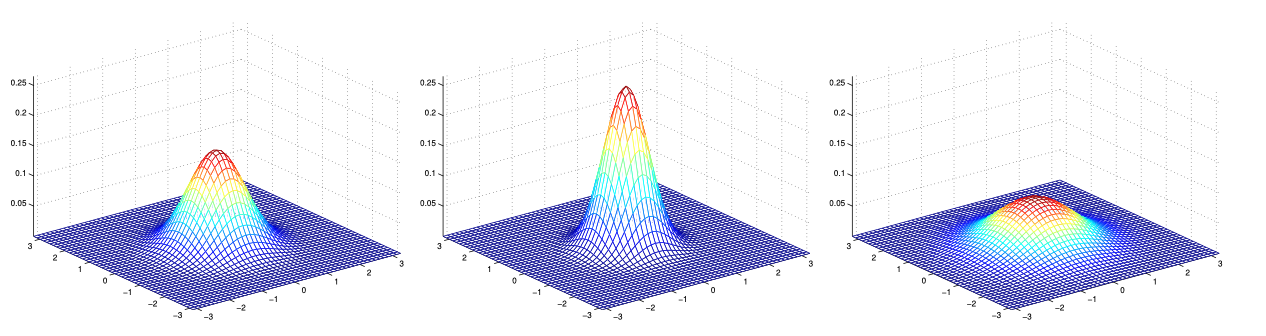
\includegraphics[scale=0.65]{img/Gaussian_Distribution.png}
\end{center}

It is true that the $n$ axes of the $(n-1)$-dimensional isocontour ellipsoid formed by an $n$-dimensional Gaussian distribution are precisely the eigenvectors of $\Sigma$ multiplied by their eigenvalues. But since we are talking about $\Sigma$'s that are symmetric and positive definite, in the $2$ dimensional case, we deal with matrices $\Sigma$ of form (up to constant scaling): 
\[\Sigma = \begin{pmatrix}
1 & \alpha \\ \alpha & 1
\end{pmatrix}\]
which has eigenvectors $(1\; 1)$ (with eigenvalue $1+\alpha$) and $(-1\;1)$ (with eigenvalue $1-\alpha$). Therefore, in the 2 dimensional case, we would be looking at Gaussian distributions that are either circular ($\Sigma = \sigma I$), ellipses angled at $45^O$ (when $\alpha > 0$ in case above), or ellipses angled at $-45^O$ (when $\alpha < 0$). The visuals are analogous for higher dimensional distributions. 

Obviously, the "peak" of the distribution will be $\mu$. 

\section{Order Statistics}
Let $X_1, X_2, ..., X_n$ be a finite collection of independent, identically distributed random variables. Suppose that they are continuously distributed with density $f$ and CDF $F$. 

\begin{definition}
Define the random variable $X_{(k)}$ to be the $k$th ranked value, called the \textit{$k$th order statistic}. This means that 
\[X_{(1)} = \min\{X_1, X_2, ..., X_n\}, \;\; X_{(n)} = \max\{X_1, X_2, ..., X_n\}\]
and in general, for any $k \in \{1, 2, ..., n\}$, 
\[X_{(k)} = X_j \text{ if } \sum_{l=1}^n \mathbb{I}_{X_l < X_j} = k - 1\]
which means that exactly $k-1$ of the values of $X_l$ are less than $X_j$. Since $F$ is continuous, 
\[X_{(1)} < X_{(2)} < ... < X_{(n)}\]
holds with probability $1$. This leads us to define the random variable $X_{(k)}$ representing the $k$th order statistic.
\[f_{(k)} (y) = \begin{cases} 
n \, {{n-1} \choose {k-1}} y^{k-1} (1-y)^{n-k} & y \in (0, 1) \\
0 & y \not\in (0,1)
\end{cases}\]
That is, $X_{(k)}$ has the Beta$(k, n-k_1)$ distribution. 
\end{definition}

\subsection{Poisson Arrival Process}
A \textit{Poisson Arrival Process} with rate $\lambda > 0$ on the interval $[0, \infty)$ is a model for the occurence of some events which may have at any time. We can interpret the process as a collection of random points in $[0, \infty)$ which are the times at which the arrivals occur. 

\textbf{Interpretation 1} Set $T_0 = 0$. The arrival times are random variables $0 < T_1 < T_2 < T_3 < ...$ such that the inter-arrival waiting times
\[W_k = T_k - T_{k-1}, \;\;\; k \geq 0\]
have the property that $\{W_k\}_{k=1}^\infty$ are independent Exp$(\lambda)$ random variables. 
\\
\\
\textbf{Interpretation 2} For any interval $I \subset [0, \infty)$, let
\[N_I \equiv \text{ number of arrivals that occur in interval } I\]
Then, $N_I \sim$ Poisson$(\lambda |I|)$, and for any collection of disjoint intervals $I_1, I_2, ..., I_n$, the random variables 
\[\{N_{I_k}\}_{k=1}^n\]
are independent. 

\begin{theorem}
These two interpretations of the arrival process are equivalent. 
\end{theorem}
\begin{proof}
In the 2nd interpretation, the statement $N_I \sim$ Poisson$(\lambda |I|)$ means that 
\[\mathbb{P}(N_I = m) = e^{-\lambda |I|} \frac{(\lambda |I|)^m}{m!}, \;\;\; m = 0, 1, 2, 3, ...\]
where $|I|$ is the length of interval $I$. From the first perspective, notice that 
\[T_k = W_1 + W_2 + ... + W_k\]
so that the $k$th arrival time $T_k$ is a sum of $k$ independent Exp$(\lambda)$ random variables. Thus, 
\[T_k \sim \text{Gamma}(k, \lambda)\]
and therefore has density
\[ \lambda e^{-\lambda t} \frac{(\lambda t)^{k-1}}{(k-1)!}, \;\;\; t>0\]
Note that the arrival times $T_i$ are not independent of each other, but the wait times $W_i$ are indeed independent. 
\end{proof}

We can slightly modify this to create a Poisson arrival process over some finite time horizon $[0, L]$. Again, you can do this two ways: 
\begin{enumerate}
    \item Starting with independent Exp$(\lambda)$ random variables $W_1, W_2, ...$, we define
    \[T_k = \sum_{i=1}^k W_i\]
    Once you have $T_k > L$, stop. 
    \item We let $N \sim$ Poisson$(\lambda L)$, since we are only working in finite interval $L$. Given $N = n$, let $U_1, U_2, ..., U_n \sim$ Uniform$([0, L])$. These define the arrival times, and let us order them to get
    \[T_k = U_{(k)}, \;\; k = 1, 2, ..., N\]
    where $U_{(k)}$ is the $k$th ordered point, with $T_1 = \min(U_1, ..., U_N)$. 
\end{enumerate}

\begin{lemma}[Memoryless Property]
The Exp$(\lambda)$ distribution has the property that for all $t, s \geq 0$, 
\[\mathbb{P}(W > t + s \; | \; W > t) = \mathbb{P}(W > s)\]
which is called the \textit{memoryless property}. We can interpret this in the following way. Let $W$ be the time you have to wait for the first arrival. Given that you already waited $t$ units of time, the probability that you have the wait $s$ additional units of time is just the probability that you wait at least $s$ from the beginning. That is, knowing that $t$ units of time have elapsed does not affect the distribution of the remaining waiting time. 
\end{lemma}

\begin{theorem}
Let $W$ be a continuously distributed random variable. Then $W \sim$ Exp$(\lambda)$ for some $\lambda > 0$ if and only if $W$ satisfies the memoryless property. 
\end{theorem}

\section{Markov Chains}
\subsection{Discrete Time Chains}
\begin{definition}
A \textit{Markov chain} is a sequence of random variables $\{X_n\}_{n=0}^\infty$, which take values in some set $\mathcal{S}$, called the \textit{state space} satisfying the \textit{Markov property}. Since we are working with discrete time chains, we will assume that $\mathbb{S}$ is a countable (and in most cases, finite). Thus, the $X_n$ will all be discrete random variables. We can also think of $X_n$ as a discrete "time" index; that is, $X_n$ is the state of the system at time $n$. Therefore, the sequence of random variables models a system evolving in a random way. 
\end{definition}

\begin{definition}
A sequence of random variables $\{X_i\}$ satisfies the \textit{Markov property} if 
\[\mathbb{P}(X_{n+1} = y \; | \; X_n = x_n, X_{n-1} = x_{n-1}, ..., X_0 = x_0\} = \mathbb{P}(X_{n+1} = y \; | \; X_n = x_n\}\]
holds for any choice oc states $y, x_n, x_{n-1}, ..., x_0 \in \mathcal{S}$ and for any $n \geq 1$. 
\end{definition}
Colloquially, given that one is at state $X_n = x_n$, knowing all the previous states does not help in predicting $X_{n+1}$. Knowing only the current state is relevant in predicting the next one. We can model this entire system using a matrix. 

\begin{definition}
Assuming that the chain is \textit{time-homogeneous}, the \textit{transition probability matrix} $P$ has elements $P_{x y}$ defined
\[P_{x y} = P(x, y) = \mathbb{P}(X_1 = y \,|\, X_0 = x) = \mathbb{P}(X_{n+1} = y \,|\, X_n = x)\]
which is the probability of moving from state $x$ to state $y$ in one step. The time homogeneous condition refers to the last equality; that is, the one-step transition probabilities don't change with the time index $n$. Note that if $\mathcal{S}$ is finite, then $P$ is a $|S| \times |S|$ matrix, and if $\mathcal{S}$ is countably infinite, then $P$ is an infinite-dimensional matrix. The axioms of probability imply that $A^T$ is an entry-wise nonnegative stochastic matrix.
\end{definition}

\begin{example}[Random Walks]
A \textit{random walk} on the integers $\mathcal{S} = \mathbb{Z}$ where a point has equal probability of moving right or left can be modeled with the probability function. 
\[P(x, y) = \mathbb{P}(X_{n+1} = y \, | \, X_n = x) = \begin{cases}
\frac{1}{2} & y = x + 1 \\
\frac{1}{2} & y = x - 1\\
0 & otherwise
\end{cases}\]
This can be generalized to multiple dimensional random walks on graphs with probability function 
\[P(x, y) = \frac{1}{\text{deg}(x)}\]
where deg$(x)$ is the number of adjacent nodes to node $x$. In this way, the point hops randomly from node to node, and if the graph is connected, then the walker can visit any vertex in the graph. 
\end{example}

\begin{example}[Discrete Moran Model]
Consider a population of size $N$. Each individual is one of two types (say, red or blue). At each time step, the system evolves in the following way: First, one of the individuals is chosen uniformly at random to be eliminated from the population; and another individual is chosen uniformly at random to produce one offspring identical to itself. These two choices are made independently. So, if a red individual is chosen to reproduce, and a blue one is chosen for elimination, then the total number of red particles increases by one and the number of blue particles decreases by one. If a red is chosen for reproduction and a red is chosen for elimination, then there is no net change in the number of reds and blues. Let $X_n$ be the number of red individuals at time $n$. The transition matrix for this chain is
\[P_{i j} = \begin{cases}
\frac{i}{N} \bigg(\frac{N-i}{N} \bigg) & j=i-1, i \neq 0 \\
\bigg(\frac{N-i}{N} \bigg) \frac{i}{N} & j=i+1, i \neq N \\
1 - 2 \bigg(\frac{N-i}{N} \bigg) \frac{i}{N} & j = i \\
0 & \text{otherwise}
\end{cases}\]
Note that the states $X_n = 0$ and $X_n = N$ are absorbing states, which represents a phenomenon called \textit{fixation}. 
\end{example}

\begin{definition}
A certain state $F$ in the state space $\mathcal{S}$ of a Markov chain is called an \textit{absorbing state} if
\[\mathbb{P}(X_{n+1} = F \; | \; X_n = F) = 1 \iff \mathbb{P}(X_{n+1} \neq F \; | \; X_n = F) = 0\]
\end{definition}

\begin{theorem}
Let there exist a time homogeneous Markov chain with transition probability matrix $P$. Given a probability distribution $\nu_n$ (a row vector) representing the a state of a system at time $t=n$, the probability distribution of which state the system will be at when $t=n+1$ can be calculated by 
\[\nu_{n+1} = \nu_n P\]
The probability distribution of the state of the system at $t=n+k$ can be calculated by summing up all of the possible probabilities that lead to each state at $t=n+k$. It is calculated equivalently as matrix multiplication: 
\[\nu_{n+k} = \nu_n P^k\]
\end{theorem}

\begin{definition}
The distribution $\nu$ of a Markov chain at time $t=0$ is called the \textit{initial distribution} for the chain. That is, $\nu$ is the initial distribution if 
\[\mathbb{P}(X_0 = x) = \nu(x)\]
\end{definition}

\begin{definition}
An \textit{invariant distribution}, or \textit{stationary distribution}, is a probability distribution $\pi$ such that 
\[\pi P = \pi\]
This means that 
\[\pi P^k = \pi\]
for all $k \in \mathbb{N}$. We can equivalently call $\pi$ the left eigenvector of matrix $P$ with eigenvalue $1$. If $\pi$ is an invariant distribution for the chain, and $X_0 \sim \pi$, then the distribution of $X_n$ does not change with $n$; it is invariant. Note that this does not mean that $X_n$ is constant; rather, it means that the distribution of $X_n$ is not changing. 
\end{definition}

\begin{example}
Let us have a two node system with nodes labeled $L$ and $R$. That is, $\mathcal{S} = \{L, R\}$. Consider a chain on this state space with transition probability matrix. 
\[P = \begin{pmatrix}
1-a & a \\ b & 1-b 
\end{pmatrix}\]
which can be visualized in the following diagram below.
\begin{center}
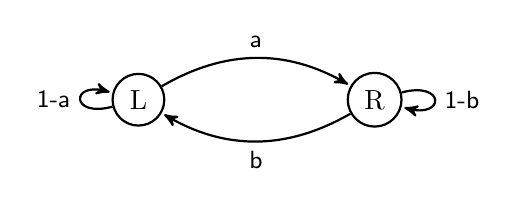
\begin{tikzpicture}[->,>=stealth',shorten >=1pt,auto,node distance=3cm,
                    thick,main node/.style={circle,draw}]
    \node[main node] (R) {R};
    \node[main node] (L) [left of=R] {L};
    \path[every node/.style={font=\sffamily\small}]
    (L) edge [loop left] node {1-a} (L)
        edge [bend left] node {a} (R)
    (R) edge [loop right] node {1-b} (R)
        edge [bend left] node {b} (L);
\end{tikzpicture}
\end{center}

Then, the stationary distribution is 
\[\pi = \Big( \frac{b}{a+b}, \frac{a}{a+b} \Big)\]
Notice that if $a = b = 0$, then this definition is ill-defined, and any probability distribution is invariant since $P = I_2$, the identity matrix. 
\end{example}

\begin{definition}
A state $x \in \mathcal{S}$ is \textit{recurrent} if
\[\mathbb{P}(X_n = n \text{ for some } n \geq 1 \, | \, X_0 = x\} = 1\]
That is, if the initial state is $x$, the chain has probability $1$ of returning to $x$ at some later time. If a state is not recurrent, then the state is said to be \textit{transient}. That is, if $x$ is transient, there is some positive probability that the chain will never return to $x$. 
\end{definition}

\begin{definition}
Two states $x, y \in \mathcal{S}$ are said to \textit{communicate}, denoted $x \leftrightarrow y$, if there are positive integers $n$ and $m$ such that 
\[P^{(n)} (x, y) > 0 \text{ and } P^{(m)} (y, x) > 0\]
That is, there is some positive probability that the chain can go from $x$ to $y$ and from $y$ to $x$ in some number of steps. 
\end{definition}

\begin{definition}
If all pairs $x, y \in \mathcal{S}$ communicate, then the chain is said to be \textit{irreducible}. If there exists a pair of states that do not communicate, then the chain is said to be \textit{reducible}. 
\end{definition}

Note that the notion of communication is an equivalence relation between states. That is, it satisfies the properties. 
\begin{enumerate}
    \item $x \leftrightarrow x$.
    \item $x \leftrightarrow y \implies y \leftrightarrow x$.
    \item $x \leftrightarrow y, y \leftrightarrow z \implies x \leftrightarrow z$.
\end{enumerate}
This relation partitions the state space $\mathcal{S}$ uniquely into transient states and irreducible sub-chains
\[\mathcal{S} = T \cup C_1 \cup C_2 \cup ...\]
More specifically, $T$ is the set of all transient states, and the sets $C_k$ are \textit{closed communication classes}, meaning that
\begin{enumerate}
    \item For all $x, y \in C_k$, $x \leftrightarrow y$. 
    \item $P(x, z) = 0$ whenever $x \in C_k$ but $z \not\in C_k$. 
\end{enumerate}
Note that for all $x, y \not\in T$, $x$ and $y$ communicate if and only if $x$ and $y$ are in the same class $C_k$. Moreover, once the chain reaches one of the sets $C_k$, it cannot leave $C_k$. 

\begin{definition}
For any state $x \in \mathcal{S}$, the \textit{period} of $x$ is defined to be
\[d(x) \equiv \gcd \{n \geq 1 \; | \; P^{(n)} (x, x) > 0\}\]
\end{definition}

\begin{theorem}
It follows that if two states $x$ and $y$ communicate, then they must have the same period: $d(x) = d(y)$. It naturally follows that if the chain is irreducible, then all states must have the same period, and we can define the period of the chain to be $d(x)$ for any $x$ we choose.
\end{theorem}

\begin{definition}
If an irreducible chain has period $1$, the chain is said to be \textit{aperiodic}. Otherwise, the chain is \textit{periodic} with period $d > 1$. 
\end{definition}

\begin{theorem}
Suppose $|\mathcal{S}| < \infty$. If the chain is irreducible, then there always exists a unique stationary distribution $\pi$. If the chain is also aperiodic, then for any initial distribution $\nu$, 
\[\lim_{k \rightarrow \infty} \nu P^k = \pi \]
Hence
\[\lim_{k \rightarrow \infty} P^{(k)}(x, y) = \pi(y)\]
for all $x, y \in \mathcal{S}$. Furthermore, for any function $F: \mathcal{S} \longrightarrow \mathbb{R}$, the limit
\[\lim_{N \rightarrow \infty} \frac{1}{N} \sum_{n=1}^N F(X_n) = \sum_{x \in \mathcal{S}} F(x)\, \pi(x) = \mathbb{E} \big( F(x) \big)\]
holds with probability $1$. In particular, the limit does not depend on the initial distribution. 
\end{theorem}
\begin{proof}
The Frobenius Extension to Perron's theorem (Linear Algebra, Theorem 7.31) combined with its applications to stochastic matrices (Linear Algebra, Theorem 7.30) proves this statement. 
\end{proof}

\begin{definition}
For each $x \in \mathcal{S}$, define the \textit{first visit} to $x$ by 
\[T_x \equiv \min\{ n \geq 1 \; | \; X_n = x\}\]
This $T_x$ is an integer-valued random variable. We say $T_x = + \infty$ if $X_n$ never reaches $x$. Then, we define the \textit{mean return time} to $x$ by 
\[\mu_x \equiv \mathbb{E}\big( T_x \, | \, X_0 = x)\]
If $x$ is transient, then $\mu_x = + \infty$, since there is positive probability that $T_x = + \infty$. 
\end{definition}

\begin{definition}
It is possible that $x$ is recurrent while $\mu_x = +\infty$. If this is the case, then $x$ is said to be \textit{null-recurrent}. If $x$ is recurrent and $\mu_x < \infty$, then $x$ is said to be \textit{positive recurrent}. 
\end{definition}

\begin{theorem}
An irreducible chain has a stationary probability distribution $\pi$ if and only if all states are positive recurrent. If a chain is irreducible and all states are positive recurrent, then 
\[\pi(x) = \frac{1}{\mu_x}\]
for all $x \in \mathcal{S}$. $\pi$ is also unique. 
\end{theorem}

\subsubsection{Exit Probabilities}
Suppose a chain is finite and irreducible. Let $a, b \in \mathcal{S}$ be given states, and let us define $h(x)$ to be the probability of hitting $b$ before $a$, given that we start from $x$. 
\[h(x) \equiv \mathbb{P} (X_n \text{ reaches } b \text{ before } a \, | \, X_0 = x)\]
Clearly, $h(b) = 1$ and $h(a) = 0$. By conditioning on the first jump out of $x$, we also have 
\begin{align*}
    h(x) & = \mathbb{P}(X_n \text{ reaches } b \text{ before } a \, | \, X_0 = x) \\
    & = \sum_{y} \mathbb{P}(X_n \text{ reaches } b \text{ before } a \, | \, X_1 = y, X_0 = x) \, \mathbb{P}(X_1 = y \,|\,X_0 = x) \\
    & = \sum_y \mathbb{P}(X_n \text{ reaches } b \text{ before } a \, | \,X_1 = y, X_0 = x) \, P(x, y) \\
    & = \sum_y \mathbb{P}(X_n \text{ reaches } b \text{ before } a \, | \,X_1 = y) \, P(x, y) \\
    & = \sum_y h(y) \, P(x, y) 
\end{align*}
The sum is over all $y \in \mathcal{S}$ for which $P(x, y) \neq 0$. This gives us a linear system of equations to solve for $h$
\begin{align*}
    & h(x) = \sum_y P(x, y) h(y) \,\, \forall x \in \mathcal{S} \setminus \{a, b\}, \\
    & h(b) = 1, \\
    & h(a) = 0
\end{align*}

\subsubsection{Exit Prize}
Let $B \subset \mathcal{S}$ be some subset of the state space, and let $g: B \longrightarrow \mathbb{R}$ be some function. Consider the function 
\[h(x) = \mathbb{E}\big( g(X_\tau) \, |\, X_0 = x \big)\]
where $\tau = \min\{ n\geq 0 \,|\, X_n \in B\}$ is the first time that the chain reaches some state in the set $B$ (this time is random). We can interpret $g(y)$ as a "prize" that is awarded if the chain first reaches $B$ at state $y$, which means that $h(x)$ is the expected prize, given that $X_0 = x$. If $x \in B$, then $\tau = 0 \implies h(x) = g(x)$. But if $x \not\in B$, then by the same argument as shown in exit probabilities, it is true that $h$ satisfies the linear system of equations
\begin{align*}
    & h(x) = \sum_g P(x, y)\,h(y), \;\; \forall x \in \mathcal{S} \setminus B, \\
    & h(x) = g(x), \;\; x \in B 
\end{align*}
Note that Exit probability system is a special case of the Exit prize system. In the former, we have defined $B = \{a, b\}$ and $g$ defined by $g(a) = 0, g(b) = 1$. 

\subsubsection{Occupation Times, Absorbing States}
Suppose that a chain on a finite $\mathcal{S}$ is irreducible. Let $B \subset \mathcal{S}$ be some subset of states and let $A = \mathcal{S} \setminus B$ be the other states. Then for $x \in A$, we wish to know how many steps the chain will take before reaching a state in the set $B$. We define 
\[\tau_B = \min\{n \geq 0 \,|\, X_n \in B\}\]
which represents the first time that $X$ is in $B$, an integer valued random variable. We wish to compute
\[h(x) = \mathbb{E}(\tau_B \,|\, X_0 = x)\]
Clearly, $h(y) = 0$ for all $y \in B$. For $x \in A$, it takes at least one step to reach $B \implies h(x) \geq 1$ for $x \in A$. We condition on the first step from $x$. This leads to the system \begin{align*}
    h(x) = 1 + \sum_{y \in \mathcal{S}} P(x, y) \, \mathbb{E}(\tau_B \,|\, X_1 = y), & \forall x \in A = \mathcal{S} \setminus B
\end{align*}
Since the chain is time-homogeneous, this means that
\begin{align*}
    h(x) = 1 + \sum_{y \in \mathcal{S}} P(x, y) \, h(y), & \forall x \in A 
\end{align*}
Since $h(y) = 0$ for all $y \in B$, we now have
\begin{align*}
    h(x) = 1 + \sum_{y \in A} P(x, y) \, h(y), & \forall x \in A 
\end{align*}
To solve this system, let us define $M$ as the $|A| \times |A|$ submatrix of $P$ obtained by keeping only the entries $P(x, y)$ with $x, y \in A$. So, the system can be written as
\begin{align*}
    h(x) = 1 + \sum_{y \in A} M(x, y) \, h(y), & \forall x \in A
\end{align*}
We can solve this system of equations through the equivalent matrix equation
\[(I - M) h = 1\]
where $1 = (1, 1, ..., 1)^T$ is the column vector consisting of all $1$'s. The solution vector is therefore
\[h = (I - M)^{-1} 1\]
So, for a particular $x \in A$, 
\[h(x) = \sum_{y \in A} (I - M)^{-1} (x, y)\]
\\

Alternatively, we can slightly modify the chain to chain $\Tilde{X}_n$ by replacing the transition probability matrix $P$ with another one defined as 
\[\Tilde{P}(x, y) = \begin{cases}
P(x, y) & x \in A, y \in \mathcal{S} \\
1 & x = y \in B \\
0 & \text{else}
\end{cases}\]
This modification means that all transitions from state in $A$ to any other state are preserved and the only transitions from a state $x \in B$ are self loops. In particular, all transitions from states $x \in B$ to states $y \in A$ are removed. Therefore, under this modified transition matrix, the states in $B$ are absorbing states. The tail sum formula implies that
\[\mathbb{E}(\tau_B \,|\, X_0 = x) = \sum_{k=0}^\infty \mathbb{P}(\tau_B > k \,|\, X_0 = x)\]
Notice that since the chain $X_n$ and $\Tilde{X}_n$ have the same transition rules before hitting a state $B$, we have 
\[P^{(k)} (x, y) = \Tilde{P}^{(k)} = M^{(k)}(x, y)\]
where $M$ is the $|A| \times |A|$ submatrix defined previously. Therefore, putting this all together, we have
\begin{align*}
    \mathbb{E}(\tau_B \,|\, X_0 = x) & = \sum_{k=0}^\infty \mathbb{P}(\tau_B > k \,|\, X_0 = x) \\
    & = \sum_{k=0}^\infty \mathbb{P}(\Tilde{X}_k \in A \,|\, X_0 = x) \\
    & = \sum_{k=0}^\infty \sum_{y \in A} \Tilde{P}^{(k)} (x, y) \\
    & = \sum_{k=0}^\infty \sum_{y \in A} M^{(k)} (x, y) \\
    & = \sum_{y \in A} \bigg( \sum_{k=0}^\infty M^{(k)} \bigg) (x, y) 
\end{align*}
Using a theorem from linear algebra, we can show that if all the eigenvalues of a $d \times d$ matrix $M$ have modulus strictly less than $1$, then $I-M$ is invertible and
\[\sum_{k=0}^\infty M^{(k)} = (I - M)^{-1}\]
where $I$ is the $d \times d$ identity matrix. If $M$ is the $|A| \times |A|$ submatrix described above, one can show that $M$ has his property and that $I - M$ is invertible. Hence, 
\[\mathbb{E}(\tau_B \,|\, X_0 = x) = \sum_{y \in A} \bigg( \sum_{k=0}^\infty M^{(k)} \bigg) (x, y) = \sum_{y \in A} (I-M)^{-1} (x, y)\]
which refers to the $(x, y)$ entry of the matrix $(I - M)^{-1}$. This is indeed consistent with our previous derivation of the formula for $h(x)$, the expected number of steps before the state reaches $B$. 

\subsection{Markov Chain Monte Carlo Algorithms}
In statistics, Markov chain Monte Carlo (MCMC) methods comprise of a class of algorithms for sampling from a probability distribution by constructing a Markov chain that has the desired distribution as its equilibrium distribution. That way, by recording samples from the chain, one may get better approximations of the actual distribution. 

Let there exist a state space $\mathcal{S}$ with some probability distribution $\pi(x)$ for every $x \in \mathcal{S}$. Clearly, 
\[\sum_{x \in \mathcal{S}} \pi(x) = 1\]
but the problem is that we do not know that $\pi$ is. We do know, however, another function $f$ that is directly proportional to $\pi$. 
\[\pi(x) = \frac{f(x)}{c}, \text{ where } c = \sum_{x \in \mathcal{S}} f(x)\]
is the normalizing constant. It is often the case that $c$ is unknown and the state space $\mathcal{S}$ is so large that computing $c$ directly is expensive. Therefore, we construct Markov chains that can provide approximations to $\pi$. 

\subsubsection{Metropolis-Hastings Algorithm}
This algorithm is useful because it does not require knowledge of the normalizing constant $c$. The algorithm only requires evaluations of 
\[\frac{\pi(x)}{\pi(y)} = \frac{f(x)}{f(y)}\]
We first have the state space $\mathcal{S}$ consisting of all the possible states. We now construct (any) probability transition matrix $q$ for a Markov chain on $\mathcal{S}$. Note that $q$ is a $|\mathcal{S}| \times |\mathcal{S}|$ matrix and $q^T$ is a stochastic matrix. This matrix is constructed by the user and is completely well-defined and known. We start off with any initial state $x_0 \in \mathcal{S}$ and iterate the following 2-steps to construct a Markov chain. 
\begin{enumerate}
    \item Given a state $X_n = x$, we generate a new state $X_{n+1}$ by first proposing a new state $y \in \mathcal{S}$ with probability $q(x, y)$ (determined from the matrix $q$). 
    \item With this chosen state $y$, we decide whether to accept to reject the proposal. With probability 
    \[\min \bigg( 1, \frac{\pi(y) \,  q(y, x)}{\pi(x) \, q(x, y)} \bigg)\]
    we accept the proposal and set $X_{n+1} = y$. Otherwise, the proposal is rejected and the new state is the same $X_{n+1} = x$. 
\end{enumerate}
Note that there are two levels of randomness here: which state the new state $y$ will be and whether to accept this state to be the next one or not. If step two did not exist (i.e. the probability of accepting the proposal is always $1$), then this would just be a regular Markov chain represented by the matrix $q$. But the addition of step 2 means that while $q$ is used in constructing the discrete chain $X_n$, it is \textit{not} the transition probability matrix of $X_n$. 

There is also a lot of flexibility on choosing $q$, although the performance of the algorithm (speed of convergence of the distribution of $X_n$ to the stationary distribution) will depend on the choice.

\begin{proposition}
For the chain defined by the Metropolis-Hastings algorithm, the distribution $\pi$ is stationary. 
\end{proposition}
\begin{proof}
Let us write in shorthand 
\[\alpha(x, y) = \frac{\pi(y)\, q(y, x)}{\pi(x)\, q(x, y)}\]
First, observe that if $x \neq y$, the transition probability for the chain defined by the algorithm is just
\[P(x, y) = q(x, y)\, \min\{1, \alpha(x, y)\}\]
Next, we claim that for all $x, y \in \mathcal{S}$, 
\[\pi(x) P(x, y) = \pi(y) \, P(y, x) \]
This condition is called \textit{detailed balance}. Assuming that $\alpha(x, y) \leq 1$, it is true that
\[\pi(x) P(x, y) = \pi(x) q(x, y) \frac{\pi(y) q(y, x)}{\pi(x) q(x, y)} = \pi(y) q(y, x)\]
In this case, we also have $\alpha(y, x) = 1 / \alpha(x, y) \leq 1$. So, 
\[\pi(y) P(y, x) = \pi(y) q(y, x) \]
and we have proved what we had claimed. Now, summing over $x$,
\[\sum_x \pi(x) P(x, y) = \sum_x \pi(y) P(y, x) = \pi(y) \sum_x P(y, x) = \pi(y)\]
since $P^T$ is stochastic. 
\end{proof}

\subsubsection{Gibb's Sampling}
Let $\mathcal{A} = \{a_1, ..., a_k\}$ be some finite set. Suppose that the state space 
\[\mathcal{S} = \mathcal{A} \times ... \times \mathcal{A} = \mathcal{A}^M\]
for some $M \in \mathbb{N}$. The following algorithm generates a Markov chain on $\mathcal{S}$ with stationary distribution
\[\pi(x) = \frac{f(x_1, x_2, ..., x_M)}{c}, \;\; x = (x_1, x_2, ..., x_M) \in \mathcal{S} \]
where $c >0$ is a normalizing constant. Note that $|\mathcal{S}| = k^M$, so computing $c$ may be expensive when $M$ is large. The current state of the chain is denoted 
\[X_n = (X_n^1, X_n^2, ..., X_n^M)\]
We think of $X_n$ as having $M$ components, each component taking values in $\mathcal{A}$. We start off with any initial state $X_0 = (X_0^1, X_0^2, ..., X_0^M)$ and construct a Markov chain by iterating the following two steps. 
\begin{enumerate}
    \item Given $X_n = (X_n^1, X_n^2, ..., X_n^M)$, we generate the next state $X_{n+1}$ by picking a component index $i \in \{1, ..., M\}$ uniformly at random. 
    \item With this chosen, well-defined $i$, we choose a random $Y^i \in \mathcal{A}$ according to the distribution
    \[\mathbb{P}(Y^i = a) = \frac{f\big(X_n^1 ,..., X_n^{i-1}, a, X_n^{i+1}, ..., X_n^M\big)}{\sum_{j=1}^k f\big(X_n^1 ,..., X_n^{i-1}, a_j, X_n^{i+1}, ..., X_n^M\big)}, \;\; a \in \{a_1, ..., a_k\}\]
    \item Then, set $X_{n+1} = \big(X_n^1, ..., X_n^{i-1}, Y^i, X_n^{i+1}, ..., X_n^M\big)$. 
\end{enumerate}
Note that at each step, only one component of $X_n$ is updated. Observe that the distribution above is also equal to 
\[\mathbb{P}(Y^i = a) = \frac{\pi\big(X_n^1 ,..., X_n^{i-1}, a, X_n^{i+1}, ..., X_n^M\big)}{\sum_{j=1}^k \pi \big(X_n^1 ,..., X_n^{i-1}, a_j, X_n^{i+1}, ..., X_n^M\big)}\]
which is the marginal distribution of the $i$th component, given the values of the other components. 

\begin{proposition}
For the chain defined by this algorithm, the distribution $\pi$ is stationary. 
\end{proposition}
\begin{proof}
We verify that the detailed balance condition holds. It is also helpful to note that $P(x, y) \neq 0$ if and only if $x$ and $y$ differ in one coordinate. 
\end{proof}

\subsection{Continuous Time Markov Chains}
As the name suggests, in a continuous time Markov chain $X_t$, the time parameter is continuous ($t \geq 0$). As before, the system jumps randomly between states in $\mathcal{S}$, but now the jumps may occur at any time and they occur randomly. This implies that there are \textit{two} sources of randomness:
\begin{enumerate}
    \item \textit{where} the system jumps and 
    \item \textit{when} the system jumps
\end{enumerate}

\begin{definition}
The Markov property in the continuous time case says that for any $s, t \geq 0$ and $y \in \mathcal{S}$, 
\[\mathbb{P}(X_{t + s} = y \, | \, X_t) = \mathbb{P}(X_{t+s} = y \, | \, X_r \; \forall 0 \leq r \leq t)\]
Colloquially, the conditional distribution of $X_{t+s}$ given the history up to time $t$ is the same as the conditional distribution of $X_{t+s}$ given only $X_t$. Thus, if we know the current state at $t$, knowing information about the past doesn't help us better predict the future state $X_{t+s}$. 
\\

In order for the Markov property to hold, the times between jumps must be exponentially distributed random variables because it is the only density that has the memoryless property. This fact has already been stated in a theorem when covering Poisson arrival processes. This is what makes Exp$(\lambda)$ so important for continuous time Markov chains. 
\end{definition}

\begin{lemma}
Let $T_1, T_2, ..., T_n$ be independent exponential random variables with rates $\lambda_1, \lambda_2, ..., \lambda_n$, respectively. Then the random variable $T \equiv \min\{T_1, T_2, ..., T_n\}$ is
\[T \sim \text{Exp}\Big(\sum_{i=1}^n T_i\Big)\]
Moreover, 
\[\mathbb{P}(T_k = \min\{T_1, ..., T_n\}) = \frac{\lambda_k}{\lambda_1 + ... + \lambda_n}\]
\end{lemma}

We can interpret the lemma above by imagining that we have $n$ alarm clocks all set simultaneously, which will ring independently at random times. Suppose that clock $k$ will ring after $T_k$ units of time have expired, where $T_k$ is a random variable distributed as Exp$(\lambda_k)$. Then, $T = \min\{T_1, ..., T_n\}$ is the time at which the first ring occurs. 

\begin{example}
The simplest and the most important continuous time Markov chains is the Poisson arrival process. The process really has a single parameter $\lambda >0$ (the rate of process) by definition and is integer valued. At each jump time, the process increases by $1$, and the time between jumps are independent, distributed as Exp$(\lambda)$. 

Notice that when $\lambda$ is large, the arrivals occur more frequently than when $\lambda$ is small, because the expected time between arrivals is $1/\lambda$. The second way we can interpret it is to choose an interval of time $t$ and let $X_t$ be the number of jumps that have occurred up to time $t$. It is a fact that $X_t$ is a integer-valued, Poisson$(\lambda t)$ distribution. That is, 
\[\mathbb{P}(X_t = k) = e^{-\lambda t} \frac{(\lambda t)^k}{k!}, \; k = 0, 1, 2, ...\]
In particular, $\mathbb{E}(X_t) = \lambda t$ and $\Var(X_t) = \lambda t$. 
\end{example}

\subsection{Branching Processes}
\begin{definition}
A \textit{branching process} is a type of Markov chain modeling a population in which each individual produces a random number of children (possibly $0$) and dies. The state space is $\mathcal{S} = \{0, 1, 2, 3, ...\}$. Furthermore, there is a discrete-time version and a continuous time version of the chain. In the discrete case, the state is $Z_n$, the size of the population at time $n = 0, 1, 2, ...$, and in the continuous case, the state is $Z_t$ for $t \geq 0$. 
\end{definition}

\subsubsection{Discrete-time Branching Process}
In the discrete case, all of the $Z_n$ individuals in the current generation branch at the same time and immediately die. The branching is independent and distributed according to the \textit{offspring distribution} $\{p_k\}_{k=0}^\infty$. Specifically, if $Z_n = m$, then 
\[Z_{n+1} = Y_1^n + Y_2^n + ... + Y_m^n\]
where $Y_i^n$ represents the number of offspring the $i$th individual in the $n$th generation has. All of them are distributed as
\[\mathbb{P}(Y_i^n = k) = p_k, \; k = 0, 1, 2, 3, ...\]
where $p_k$ is the probability that a parent has $k$ children. Note that if $p_0 \neq 0$, then there is positive probability that $Y_i^n = 0$ for all $i$, meaning that the population can go extinct. A sample branching process up to the second generation is shown below. 
\begin{center}
\begin{tikzpicture}[scale=0.8]
    \draw[fill] (0,4) circle (0.05);
    \draw[fill] (-2,2) circle (0.05);
    \draw[fill] (0,2) circle (0.05);
    \draw[fill] (2,2) circle (0.05);
    \draw[dashed] (0,4)--(-2,2);
    \draw[dashed] (0,4)--(0,2);
    \draw[dashed] (0,4)--(2,2);
    \draw[fill] (-3,0) circle (0.05);
    \draw[fill] (-1,0) circle (0.05);
    \draw[dashed] (-2,2)--(-3,0);
    \draw[dashed] (-2,2)--(-1,0);
    \draw[dashed] (2,2)--(3,0);
    \draw[dashed] (2,2)--(1,0);
    \draw[dashed] (2,2)--(2,0);
    \draw[fill] (3,0) circle (0.05);
    \draw[fill] (2,0) circle (0.05);
    \draw[fill] (1,0) circle (0.05);
    \node at (5,4) {$Z_0 = 1$};
    \node at (5,2) {$Z_1 = 3$};
    \node at (5,0) {$Z_2 = 5$};
    \draw[->] (4.3,4)--(3.5,4);
    \draw[->] (4.3,2)--(3.5,2);
    \draw[->] (4.3,0)--(3.5,0);
    \node at (-5, 3) {$Y_1^0 = 3$};
    \node at (-5, 1.5) {$Y_1^1 = 2$};
    \node at (-5, 1) {$Y_2^1 = 0$};
    \node at (-5, 0.5) {$Y_3^1 = 3$};
\end{tikzpicture}
\end{center}

Suppose that the mean number of offspring of a single parent is finite. 
\[\mu = \mathbb{E}(Y) = \sum_{k=0}^\infty k \, \mathbb{P}(Y = k) = \sum_{k=0}^\infty k \, p_k < \infty\]
If $Y_1$ and $Y_2$ are two independent, discrete random variables, we can define their convolution and use the fact that $\mathbb{P}(Y_i = k) = p_k$ to get
\begin{align*}
    \mathbb{P}(Y_1 + Y_2 = k) & = \sum_j \mathbb{P}(Y_1 = k - j) \, \mathbb{P}(Y_2 = j) \\
    & = \sum_{j=0}^\infty p_{k-j} p_j, \;\; k = 0, 1, 2, ...
\end{align*}
This is a two-fold convolution of the sequence $\{p_k\}$ with itself, denoted
\[p_k^{*2} = \sum_{j=0}^\infty p_{k-j} \, p_j\]
Extending this, we can find the $m$-fold convolution of the sequence $\{p_j\}$ with itself, represented by the sequence $\{p_j^{*m}\}$, where $p_k^{*m}$ is the $k$th term in this sequence. This gives us
\[p_k^{*n+1} = \sum_{j=0}^\infty p_{k-j} \, p_j^{*n}\]
for all $n \in \mathbb{N}$. Using this, we can write down the transition probabilities for the Markov chain $Z_n$. 
\[\mathbb{P}(Z_{n+1} = k \, | \, Z_n = m) = \begin{cases}
0 & \text{if } m = 0 \\
p_k^{*m} & \text{if } m \geq 1, k \geq 0
\end{cases}\]
where $\mathbb{P}(Z_{n+1} = k \, | \, Z_n = m)$ represents the probability of the $n$th generation consisting of $m$ individuals producing a total of $k$ offspring for the $(n+1)$th generation. Thus, the branching process is completely determined by the distribution of $Z_0$ and the offspring distribution $\{p_k\}_{k=0}^\infty$. 

\begin{lemma}
Given this discrete-time branching process, let $\mu$ be the mean of the offspring distribution. Then, 
\[\mathbb{E}(Z_n \, | \, Z_0 = 1) = \mu^n\]
If $\mu > 1$, the mean of $Z_n$ grows exponentially, and if $\mu_1$, the mean of $Z_n$ decreases exponentially. 
\end{lemma}

\subsubsection{Continuous-time Branching Process}
A continuous time branching process $Z_t$ has very similar structure to the discrete time branching process, except that the times between branch events (for each individual) are independent exponentially distributed random variables Exp$(\lambda)$, where the parameter $\lambda> 0$ is the branching rate. It is as though each individual has an independent alarm clock which rings as a time that is Exp$(\lambda)$, independently of all other clocks. So, if there are currently $N$ individuals, then the next alarm will ring at rate $\lambda N$; that is, the time until the next ring is distributed as Exp$(\lambda N)$, since it is the minimum of $N$ independent Exp$(\lambda)$ random variables. When an individual branches (clock rings), that individual produces a random number of offspring, according to the offspring distribution $\{p_k\}$, as before. So, a continuous time branching process has the same geneological structure as the discrete time process, but the times between branch events is randomized. Consequently, whether or not the process eventually goes extinct, depends only on the offspring distribution, not on the branching rate $\lambda$. 

Let $m_1(t) = \mathbb{E}(Z_t)$ denote the expected population size at time $t$. Then, it is a fact that $m_1(t)$ satisfies the ordinary differential equation
\[\frac{d}{d t} m_1 (t) = \lambda(\mu - 1) m_1 (t)\]
where 
\[\mu = \sum_{k=1}^\infty k p_k\]
is the mean of the offspring distribution. Solving this equation reveals that 
\[m_1 (t) = e^{\lambda (\mu-1) t} m_1 (0)\]
If $\mu > 1$, the mean population size grows exponentially, and if $\mu < 1$, the mean population size decreases exponentially. 

\subsubsection{Extinction Probability, Generating Functions}
The expression for the transition probabilities of $Z_n$ (disrete case) is quite difficult to work with. Alternatively, it can be convenient to work with generating functions. 

\begin{definition}
The \textit{generating function} for the offspring distribution is the function 
\[G(s) \equiv \sum_{k=0}^\infty p_k \, s^k = \mathbb{E}(s^Y)\]
where $Y \sim \{p_k\}$ is a random variable representing the number of children produced by a given individual. Note that $G$ is a power series that simply encodes information about the offspring distribution (also a sequence) $\{p_k\}_{k=0}^\infty$. 
\end{definition}

\begin{theorem}
\begin{enumerate}
    \item The radius of convergence of $G(s)$ is at least $1$. $G(s)$ defines a continuous function on $|s| \leq 1$. 
    \item On the interval $[0,1]$, $G(s)$ is increasing and convex. If $p_0 + p_1 < 1$, then $G(s)$ is strictly convex for $s \in [0,1]$. 
    \item $G(0) = p_0$. 
    \item $G(1) = 1$. 
    \item $G^\prime(1^-) = \mu$ is the expected number of offspring of a single individual. 
\end{enumerate}
\end{theorem}
\begin{proof}
We use the fact that 
\[\sum_{k=0}^\infty p_k = 1 \text{ and } 0 \geq p_k \geq \; \forall k = 0, 1, 2, ...\]
\end{proof}

\begin{theorem}
Suppose that $Z_0 = 1$ and that $p_0 + p_1 < 1$. Then
\[\lim_{n \rightarrow \infty} \mathbb{P}(Z_n = 0) = \mathbb{P}(\text{eventual extinction}) = t\]
where $t \in [0, 1]$ is the smallest non-negative root of the equation $t = G(t)$. If $\mu \leq 1$, then $t = 1$ (clearly, since the population will exponentially decrease on average). If $\mu > 1$, there is a positive probability that the population never goes extinct. 
\end{theorem}
\begin{proof}
Let $t$ be the probability that an individual's descendent family tree goes extinct. That is, $t = \mathbb{P}(Z_n = 0$ for some $n \geq 1 \; | \; Z_0 = 1)$. To derive the equation $t = G(t)$, let us condition on the first generation, with $Y_1$ denoting the number of offspring of the single parent. 
\begin{align*}
    t & = \mathbb{P}(\text{eventual extinction} \; | \; Z_0 = 1) \\
    & = \sum_{k=0}^\infty \mathbb{P}(\text{eventual extinction} \; | \; Z_0 = 1, Y_1 = k) \, \mathbb{P}(Y_1 = k \; | \; Z_0 = 1) \\
    & = \sum_{k=0}^\infty \mathbb{P}(\text{eventual extinction} \; | \;Z_0 =1, Y_1 = k) \, p_k
\end{align*}
That is, given that there are $k$ children of the first individual, the probability that this first individual's descendent family tree will go extinct is equal to the probability that each of the $k$ children's trees go extinct. These $k$ extinction events are independent. Therefore, 
\[\mathbb{P}(\text{eventual extinction} \; | \;Z_0 = 1, Y_1 = k) = t^k\]
which implies that 
\[t = \sum_{k=0}^\infty \mathbb{P}(\text{eventual extinction} \; | \; Z_0 = 1, Y_1 = k) \, p_k = \sum_{k=0}^\infty t^k \, p_k = G(t)\]
Additionally, under the hypothesis that $p_0 + p_1 < 1$, then $G(s)$ is strictly convex on $[0,1]$. Hence if $G^\prime (1) = \mu \leq 1$, the smallest non-negative root of $t = G(t)$ must be $t=1 \implies$ extinction occurs with probability 1. On the other hand, if $G^\prime (1) = \mu > 1$, then the smallest root of $t = G(t)$ occurs in the interval $[0,1)$. 
\end{proof}

Note that this result applies to both the discrete time case and the continuous time case. In continuous-time chains, whether or not the population goes extinct does not depend on $\lambda$, the rate at which individuals give birth. The $\lambda$ affects the time at which extinction occurs (if it occurs), but it does not affect the probability that it occurs. However, the extinction probability certainly does depend on the offspring distribution. 

\begin{definition}
A random variable $X$ is a \textit{counting variable} if it takes values in $\{0, 1, 2, ...\}$. 
\end{definition}

Note that generating functions is a mapping from $X$, the set of counting variables (all assumed to be pairwise independent) to the algebra of power series over variable $s$.
\[G: X \longrightarrow F[[s]]\]

\begin{lemma}
Let $X$ and $Y$ be two independent random counting variables, with generating functions $G_X (s) = \mathbb{E}(s^X)$ and $G_Y (s) = \mathbb{E}(s^Y)$. Then, the generating function for the random variable $Z = X + Y$ is $G_Z(s) = G_X (s) G_Y (s)$. That is, the generating function mapping $G$ is a homomorphism that maps addition to multiplication. In particular, if $X$ and $Y$ are iid, then $G_Z (s) = G_X (s)^2$. 
\end{lemma}
\begin{proof}
Since $X$ and $Y$ are independent, 
\[G_Z (s) = \mathbb{E}(s^Z) = \mathbb{E}(s^{X+Y}) = \mathbb{E}(s^X s^Y) = \mathbb{E}(s^X) \mathbb{E}(s^Y) = G_X (s) G_Y (s)\]
\end{proof}

Applying this argument iteratively, we get the following lemma. 
\begin{lemma}
Let $N \geq 1$ be a fixed positive integer. Let $Y_1, Y_2, ..., Y_N$ be independent, identically distributed random counting variables with generating function $G_Y (s) = \mathbb{E}(s^Y)$. Then, the generating function for the sum $Z = Y_1 + ... + Y_n$ is 
\[G_Z (s) = G_Y (s)^N\]
\end{lemma}

Now, suppose that $N$ is not fixed, but another random variable. We wish to describe the distribution of the sum of a random number of random variables. 

\begin{lemma}
Let $Y_1, Y_2, Y_3, ...$ be a collection of independent, identically distributed random variables with generating function $G_Y (s) = \mathbb{E}(s^Y)$. Let $N$ be a random counting variable, independent of the $Y_i$. Let $N$ have generating function $G_N (s)$. Then the generating function for $Z = Y_1 + Y_2 + ... + Y_N$ is 
\[G_Z (s) = G_N \big( G_Y (s) \big)\]
\end{lemma}
\begin{proof}
Just condition on $N = k$ 
\begin{align*}
    G_Z (s) = \mathbb{E}(s^Z) & = \sum_{k=0}^\infty \mathbb{E}\big( s^Z \,|\, N=k\big) \, \mathbb{P}(N=k) \\
    & = \sum_{k=0}^\infty \mathbb{E}(s^{Y_1 + ... + Y_k} \,|\,N=k) \, \mathbb{P}(N=k) \\
    & = \sum_{k=0}^\infty G_Y (s)^k \, \mathbb{P}(N=k) \\
    & = \mathbb{E}\big( G_Y (s)^N \big) = G_N \big( G_Y (s) \big)
\end{align*}
\end{proof}

\begin{theorem}
Let $G(s)$ be the generating function for the offspring distribution $G(s) = \sum_{k=0}^\infty p_k s^k$. Suppose that $Z_0 = 1$ and let $G_n (s) = \mathbb{E}(s^{Z_n})$ be the generating function for the random variable $Z_n$. Then, 
\[G_{n+m} (s) = G_n \big(G_m (s)\big) = G_m \big( G_n (s) \big)\]
Hence, 
\[G_n (s) = G(G(G(...(G(s))...))) \;\;\;\; \text{n-fold composition}\]
\end{theorem}

\begin{example}
Suppose the offspring distribution is
\[p_k = q p^k, \;\; k \geq 0\]
for some $p \in (0, 1)$, where $q = 1-p$. Thus, the number of children from a given parent is $Y = X - 1$, where $X \sim$ Geom$(q)$. Then, $\mathbb{E}(Y) = \frac{1}{q} - 1 = \frac{p}{q}$. With some computation, this means that
\[G(s) = \frac{q}{1- p s}\]
and $t = \min \{1, \frac{q}{p}\}$. 
\end{example}

\end{document}
